\documentclass[11pt]{article}
\usepackage[utf8]{inputenc}
\usepackage{amsmath,amssymb}
\usepackage{graphicx}
\usepackage{booktabs}
\usepackage{array}
\usepackage{tabularx}
\usepackage{hyperref}
\usepackage{geometry}
\geometry{margin=1in}
\emergencystretch=3em
\newcolumntype{Y}{>{\raggedright\arraybackslash}X}
\newcolumntype{L}[1]{>{\raggedright\arraybackslash}p{#1}}

\title{PolitiKAST: Political Knowledge-Augmented Multi-Agent Simulation of Voter Trajectories for Korean Local Elections}
\author{Seongjin Lee\\BHSN}
\date{Draft -- \today}

\begin{document}

\maketitle

\begin{abstract}
This paper proposes a validation-first multi-agent simulation framework that combines large language models (LLMs), a synthetic Korean population, and a political knowledge graph (KG) to evaluate whether voter-agent simulations can reproduce held-out opinion-poll trajectories before making any election-outcome claim. Each voter is represented as a persona endowed with rich socio-demographic attributes and baseline political preferences, constructed from a synthetic population dataset aligned with official Korean statistics. Time-varying information environments---including news coverage, scandal investigations, court decisions, spokesperson briefings, and published opinion polls---are represented as an event-centric political KG grounded in an election ontology and a discourse ontology. Voter agents are implemented as a thin custom LLM-agent layer backed by \texttt{LLMPool}/LiteLLM; they query relevant slices of the KG and update their utilities for parties and candidates over time. We derive an intuitive yet expressive mathematical model that jointly captures (i) media and scandal valence effects, (ii) bandwagon and underdog reactions to public poll exposure, (iii) second-order election dynamics driven by government approval, (iv) correlated choices across multiple ballot positions, and (v) an explicit separation between persona-level traits and shared political context encoded in the KG. The framework defines a rolling-origin validation pipeline: official election-poll releases during the six-month pre-election window are split into time-ordered calibration and validation targets, and later polls are scored only from information available before their fieldwork or publication cutoff. Crucially, official poll results are hidden calibration and validation labels rather than default voter-agent prompt context; after a configuration is frozen, inference consists of injecting source-backed or hypothetical event sequences into the KG/scenario state and comparing the resulting counterfactual trajectories. A clean no-cache validation gate has been run for the three available official pre-election poll targets across two stages: a baseline $n{=}200$ clean run that fails leader agreement with large errors in all three regions, and a post-enrichment R6 full run after KG Track A (Person/Source political narrative) and Track B (generational/gender CohortPrior nodes) are ingested and the voter prompt is extended with a cohort prior block. After enrichment, all three rated regions achieve leader agreement, mean MAE improves from $0.5066$ to $0.1782$ ($2.84\times$ tighter), and Daegu mayor in particular reaches a near-PASS at MAE $0.0538$ without any region-specific scenario hardcode. Seoul mayor maintains leader agreement but misses the strict MAE gate due to a documented cohort-prior over-amplification at $n{=}200$. Gwangju and Daegu Dalseo remain unavailable for official-poll validation. This draft therefore reports a partially passed validation gate (leader agreement for $3/3$ rated regions, near-PASS MAE for $1/3$) as a calibration trajectory and introduces the counterfactual inference protocol rather than claiming a successful 2026 election forecast.
\end{abstract}

\section{Introduction}

Forecasting elections has long been a central task in political science and political communication, with approaches ranging from structural macro models to polling-based nowcasts and expert judgment. Recent advances in large language models (LLMs) and multi-agent systems have opened a new line of work: simulating artificial electorates comprised of thousands or millions of programmatic agents that consume information, form preferences, and cast votes in silico. This paradigm promises richer counterfactual analysis (\emph{what if this scandal had not occurred?}) and more fine-grained explanations of voting behavior than traditional aggregate models.

Korean local elections provide a particularly compelling testbed. Voters often cast ballots for multiple positions (e.g., metropolitan mayor, district head, local council, superintendent), and these choices are neither fully independent nor fully identical. Local races are influenced by national-level dynamics such as presidential approval and ``government punishment'' considerations, but also by local issues, candidate valence, campaign events, and interactions among these factors. Local and by-elections are therefore modeled as second-order contests with lower turnout and protest-vote incentives~\cite{reif1980secondorder}. Moreover, media coverage, corruption allegations, prosecutorial investigations, and court decisions can shift candidate reputations over the campaign, while repeated opinion polls both measure and shape voter expectations.

A key limitation of many existing approaches is that they either (i) treat voters as homogeneous aggregates, ignoring micro-level heterogeneity, or (ii) treat each voter as an isolated agent with all relevant information folded into latent utilities, without an explicit, shareable representation of the political context. In contrast, this paper advocates a dual-layer architecture in which: (a) each voter is a rich persona aligned with demographic statistics, and (b) the shared political environment is represented as a structured knowledge graph capturing elections, candidates, parties, issues, events, and polls.

This paper makes four contributions:
\begin{itemize}
  \item It defines a formal problem setting for modeling Korean local elections as multi-position choice tasks under a dynamic information environment, with personas drawn from a synthetic population and shared context encoded in a political KG.
  \item It introduces a utility-based model in which voter preferences are decomposed into baseline components, media and scandal valence shocks, poll feedback effects, and government approval terms, augmented by a KG-based information state that determines which events and frames each persona is exposed to.
  \item It specifies a concrete data and storage architecture for integrating a large Korean synthetic persona dataset, relational election and poll tables, an event-centric KG, and a time-bounded retrieval corpus, including a poll consensus layer that aggregates heterogeneous polls into temporally smooth support estimates.
  \item It outlines an \texttt{LLMPool}/LiteLLM-backed multi-agent implementation and a validation-first experimental design that calibrates on earlier official poll releases, validates on later held-out poll releases, hides those poll labels from voter prompts by default, and then runs frozen-parameter counterfactual inference over event-KG interventions under a temporal information firewall.
\end{itemize}

The immediate goal is not zero-shot election prediction or poll-fed nowcasting. This draft is intended as a protocol and harness report for fitting a KG-augmented, persona-based election simulation framework to hidden official polling labels, validating against later hidden labels, freezing the resulting configuration, and then using the simulator for event-driven counterfactual prediction such as candidate withdrawal, nomination, scandal, or endorsement scenarios.

\begin{figure}[t]
\centering
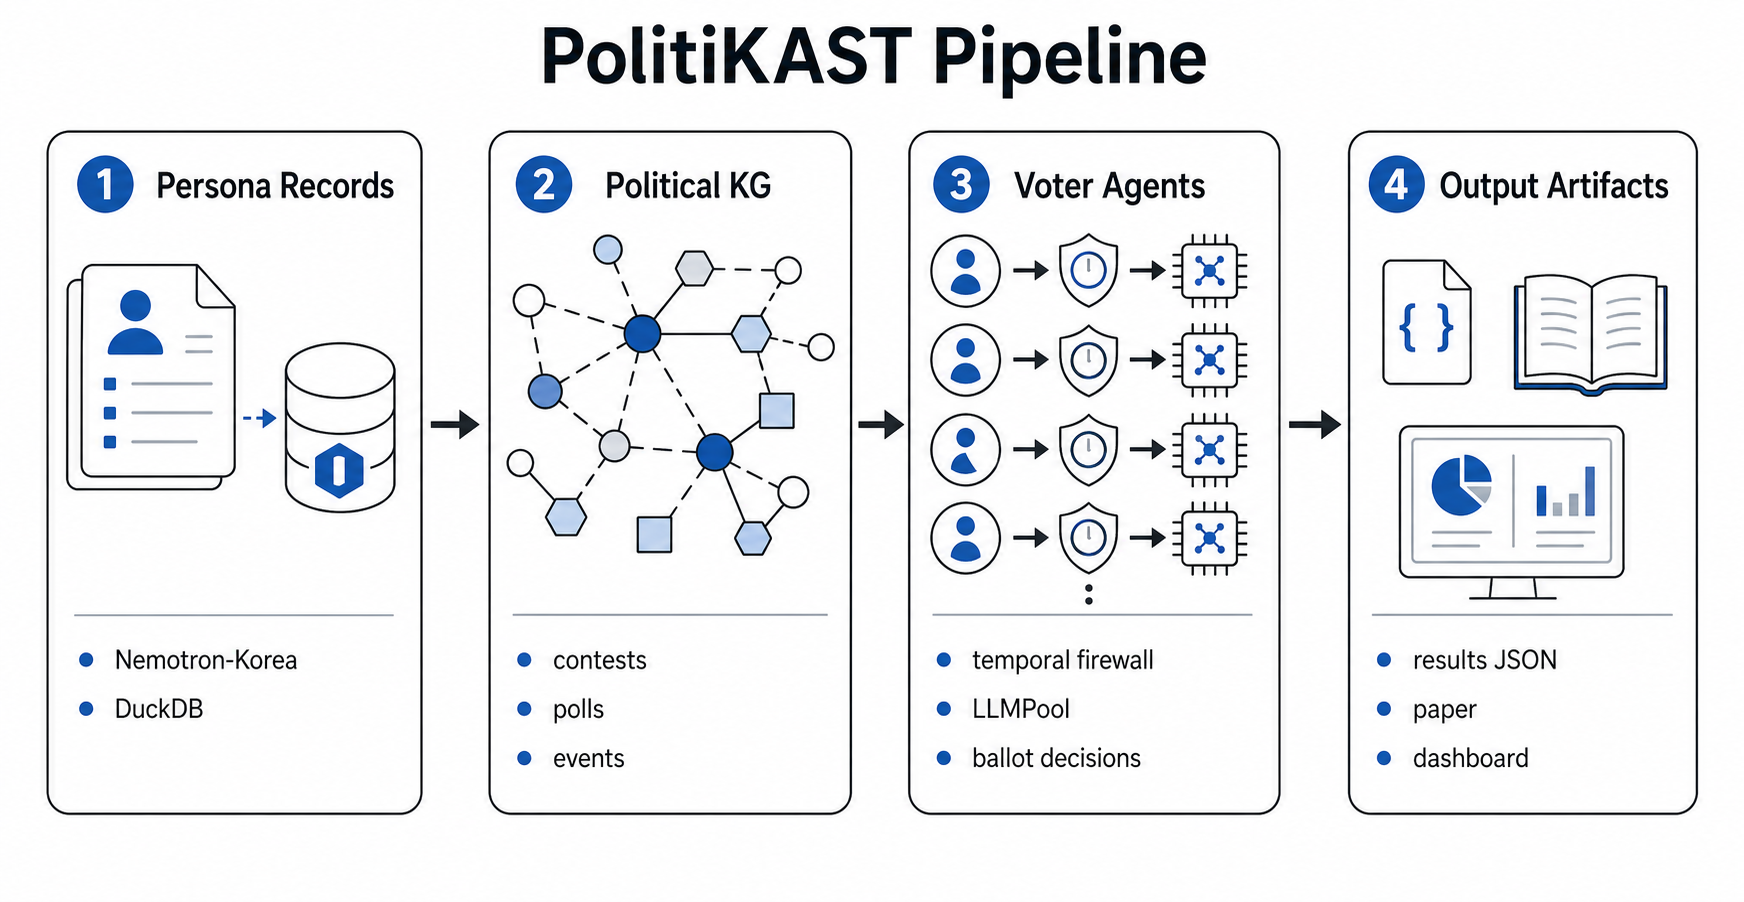
\includegraphics[width=\linewidth]{assets/fig_pipeline_architecture_ai.png}
\caption{PolitiKAST end-to-end pipeline. Static persona records and relational election tables provide the voter and contest substrate; the political KG, temporal firewall, and LLMPool-backed voter agents generate time-bounded ballot decisions and downstream artifacts.}
\label{fig:pipeline-architecture}
\end{figure}

\section{Background and Related Work}

\subsection{Media, Scandals, and Political Communication}

A large literature documents how political scandals and media coverage affect electoral outcomes. Empirical studies find that candidates involved in scandals typically suffer reduced vote shares and lower re-election probabilities, with effects modulated by scandal severity, media attention, and the broader news environment. Scandals tend to have front-loaded impacts that decay over time, and their consequences depend on partisanship and prior beliefs. We treat scandal effects as probabilistic penalties because meta-analytic evidence finds vote losses but ambiguous turnout effects~\cite{solaz2018scandalmeta}.

Beyond scandals, strategic communication by parties and governments---including spokesperson briefings and press conferences---frames issues and shapes perceived candidate valence. The interaction between media congestion, issue competition, and scandal potential influences whether particular events resonate with voters or are overshadowed by competing stories.

\subsection{Opinion Polls, Bandwagon and Underdog Effects}

Opinion polls play a dual role in electoral dynamics. On the one hand, polls measure current support levels with sampling error and method-specific biases. On the other hand, published poll results can produce behavioral responses such as bandwagon effects (voters joining the perceived winner) or underdog effects (voters rallying to trailing candidates). Field and survey experiments show that poll information can shift late-deciding and weakly attached voters, though effect sizes and directions vary across contexts. The default prior favors bandwagon over underdog effects because survey-experimental evidence finds consistent bandwagon effects and no underdog evidence~\cite{hansen2016polls}.

The relation between polls and final election outcomes is therefore endogenous: polls reflect voter preferences, but also feed back into the information environment and voter expectations. Any simulation that aims to forecast both polls and elections must explicitly model this feedback loop.

\subsection{Second-Order Elections and Government Punishment}

The ``second-order election'' thesis argues that subnational or supranational elections (e.g., local, regional, European Parliament) are often used by voters to reward or punish the national government rather than to decide directly on local issues. Empirically, governing parties tend to perform worse in midterm or lower-salience elections, and government approval levels are strong predictors of local election results. In the Korean context, mixed-member electoral systems and local elections provide a rich setting where institutional design, strategic voting, and government evaluation interact. Korean voters can exhibit strategic voting even when proportional and district ballots coexist~\cite{choi2006strategic}.

\subsection{Split-Ticket Voting in Korean Elections}

Split-ticket voting is widely observed in mixed-member and multi-level electoral systems. Korean studies show that split-ticket behavior is associated with weaker partisanship, specific socio-demographic profiles, and evaluations of government performance. Voters may support one party in constituency races and another in proportional or local contests, reflecting both national and local considerations. The split-ticket transition prior is justified by evidence that about 20 percent of Korean voters split their district and party-list votes in 2004~\cite{splitticket_korea}.

These findings motivate a model in which all ballot positions share common latent factors (ideology, party affinity, government approval), but also include race-specific components and idiosyncratic variation. The correlation structure across positions is essential for capturing realistic patterns of straight-ticket and split-ticket voting.

\subsection{Agent-Based Election Forecasting}

Agent-based models (ABMs) of elections represent voters as individual agents with preferences and social ties, simulating campaign dynamics and turnout over time. Recent work shows that ABMs can successfully forecast real elections by calibrating agent-level parameters to polls and past results, including live predictions of general elections. Agent-based election forecasting is useful because individual voters are otherwise mostly absent from aggregate forecasting exercises~\cite{gergaud2022abmelections}. Such models typically rely on relatively simple behavioral rules and low-dimensional voter attributes due to computational constraints.

\subsection{LLM-Based Voting and Multi-Agent Frameworks}

Recent research on LLM Voting investigates how LLM agents make choices in voting scenarios, how their collective decisions compare to human preferences, and how prompts and decision rules influence outcomes. While these studies do not directly simulate full electorates, they demonstrate that language models can approximate structured decision-making under varying information and framing conditions, while ballot order, persona specification, and temperature can shift LLM collective outcomes~\cite{yang2024llmvoting}. ElectionSim demonstrates million-level LLM voter simulation for U.S. presidential scenarios~\cite{liu2024electionsim}, whereas PolitiKAST focuses on Korean local elections with KG-grounded temporal context.

On the engineering side, multi-agent libraries such as CAMEL provide abstractions for creating, orchestrating, and scaling large populations of interacting LLM agents. CAMEL offers primitives for defining agent roles, societies, and communication patterns, as well as tools for integrating external data and tools. This framework is a natural foundation for building election simulation engines that leverage LLMs for micro-level decisions while retaining explicit control over macro-level structure and parameters.

\subsection{Synthetic Personas for Korean Agents}

Synthetic population datasets built from official statistics and administrative data enable micro-simulation of policy and electoral scenarios without relying on identifiable personal data. For the Korean context, recent work has released large-scale persona datasets aligning millions of synthetic individuals with demographic distributions (region, age, gender, occupation, income, household type) derived from national statistics and related sources. These datasets expose both tabular attributes and multiple persona narratives per individual, and are well suited as the base agent pool for LLM-based election simulations~\cite{bhattacharjee2024nemotron}.

\subsection{Political Ontologies and Knowledge Graphs}

Election and political ontologies provide structured vocabularies for modeling elections, contests, parties, candidates, districts, and results. The KG schema reuses election concepts such as election, candidacy, electorate, constituency, party, and result, aligned with public election ontology practice~\cite{ukparl_election_ontology}. Event-centric knowledge graphs built from news have been used to represent political events, actors, and issues, enabling complex queries and visual analytics.

More recently, political discourse ontologies and knowledge graphs have been proposed to represent speeches, debates, and media narratives as structured entities linked to issues, frames, and actors. Newsroom-oriented KG platforms show how journalistic workflows can be supported by entity and event linking. This work informs the design of the political KG in our framework: elections and institutions provide the structural backbone, while events and narratives populate the temporal dimension.

\section{Data and Storage Architecture}

\subsection{Persona Layer: Relational Core + Narrative Text}

\paragraph{Synthetic Population.}
We use Nemotron-Personas-Korea~\cite{bhattacharjee2024nemotron} (CC BY 4.0), an NVIDIA-released synthetic population of \textbf{1{,}004{,}752 records yielding $\sim$7M persona descriptions}, grounded in South Korean demographic and geographic distributions. Each record exposes 26 fields: seven narrative persona fields, six free-form attribute fields, twelve demographic/geographic fields covering 17 provinces and 252 administrative districts, and a UUID primary key. The dataset includes only adults aged 19 and above; its construction relies on a probabilistic graphical model (PGM) that assumes conditional independence between several demographic factors when sampling fine-grained occupations. We discuss the resulting limitations in Section~\ref{sec:limitations}.

\begin{figure}[t]
\centering
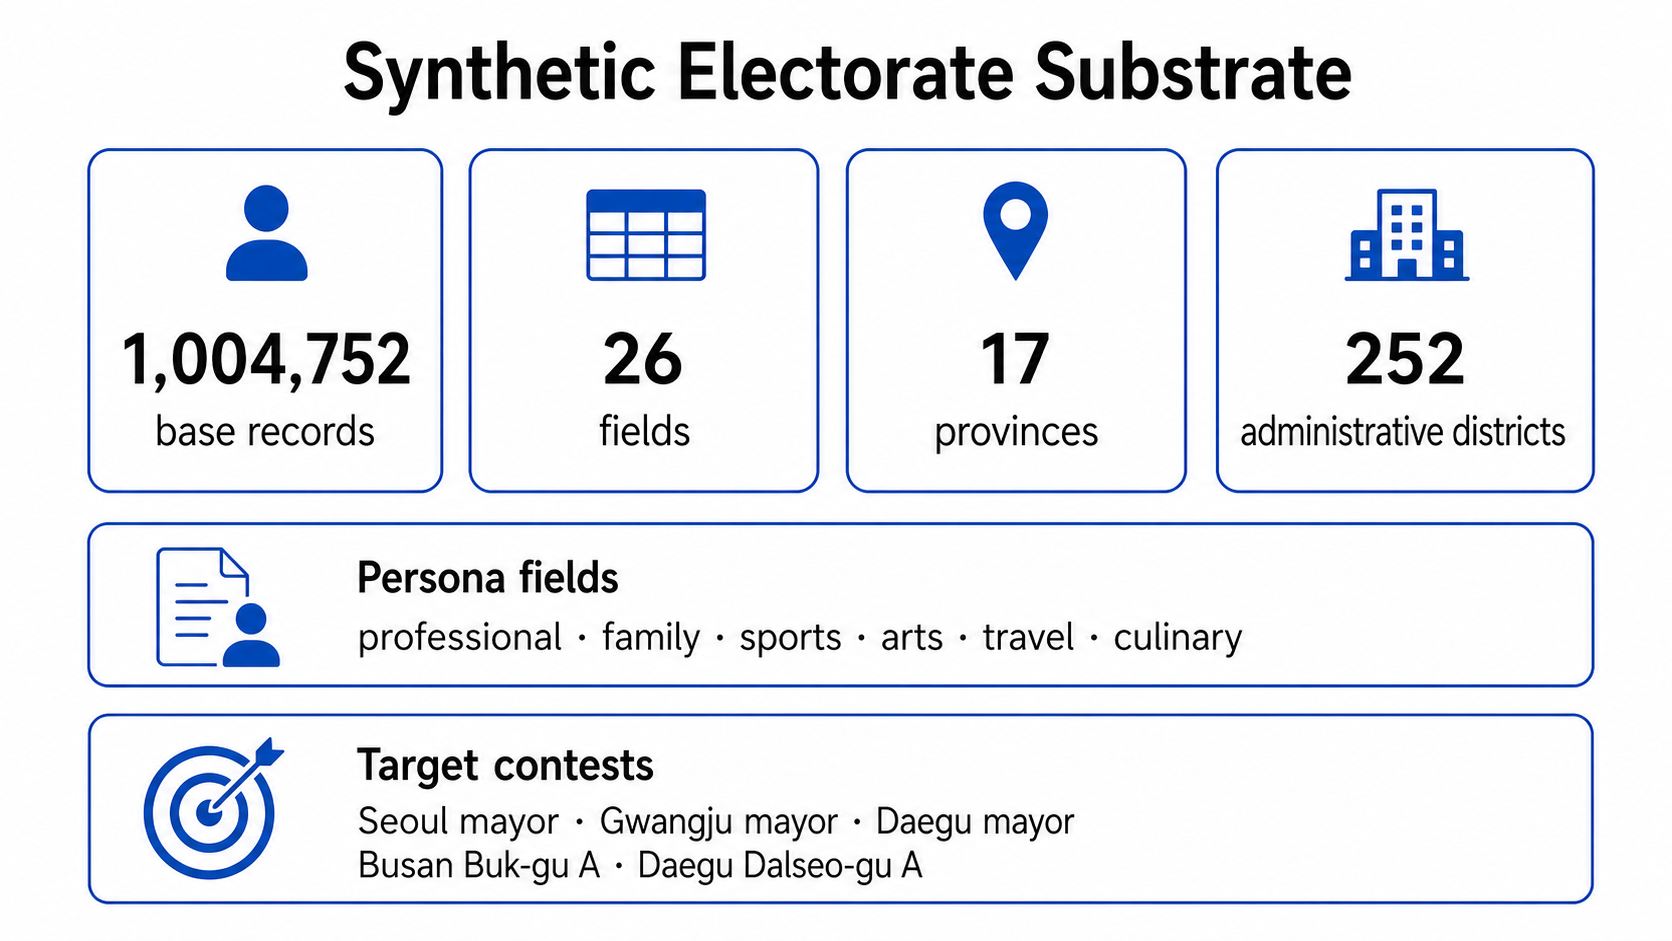
\includegraphics[width=0.92\linewidth]{assets/fig_persona_data_card_ai.png}
\caption{Persona-layer data card for Nemotron-Personas-Korea. The card records only source-published dataset properties used by the simulator design and highlights the adults-only coverage limitation relevant to Korean voting-age simulations.}
\label{fig:persona-data-card}
\end{figure}

The dataset is read from local Parquet files (9 shards) and ingested into DuckDB. Each record provides both tabular attributes and multiple persona narratives. To support efficient sampling, joining, and aggregation, we store persona data in two relational tables:

\begin{itemize}
  \item \textbf{persona\_core}: a row per persona with columns for demographic and geographic attributes, such as
  \begin{itemize}
    \item \texttt{uuid} (primary key), \texttt{province}, \texttt{district}, \texttt{sex}, \texttt{age}, plus marital, military, family, housing, education, field-of-study, and occupation attributes.
  \end{itemize}
  \item \textbf{persona\_text}: a row per persona with long-text narrative fields, such as
  \begin{itemize}
    \item Core, professional, family, travel, culinary, arts, and sports persona narratives, plus cultural background, skills, hobbies, and career-goal text fields.
  \end{itemize}
\end{itemize}

This design reflects the tabular structure of the underlying dataset and enables efficient indexing on region and demographics for stratified sampling and aggregation. Narrative fields are injected into voter-agent prompts as needed but are not required for most database queries. The current harness treats the persona source as adults-only and records this as a limitation because the Korean voting age includes 18-year-old voters.

\subsection{Election and Result Tables}

Election structure and results are stored in a relational schema including tables such as:

\begin{itemize}
  \item \textbf{election}: metadata for each election (type, year, scope).
  \item \textbf{contest}: a row per ballot position (e.g., metropolitan mayor, district mayor), including election, district, and office.
  \item \textbf{party}: party identifiers and attributes.
  \item \textbf{candidate}: candidate identifiers, party links, incumbency, and biographical features.
  \item \textbf{result}: realized vote counts and shares by contest, candidate, and district.
\end{itemize}

These tables form the structural backbone that the KG layer references.

\subsection{Poll Data: Raw Archive and Consensus Layer}

Opinion polls are stored in two layers.

\paragraph{Raw poll archive.} Each poll release is stored in a \textbf{raw\_poll} table with columns such as pollster, sponsor, mode (phone, ARS, online, in-person), fieldwork dates, sample size, response rate, and published time. Poll-specific results are stored in a \textbf{raw\_poll\_result} table with one row per poll--candidate--contest triple.

\paragraph{Consensus poll layer.} Raw polls vary by pollster, methodology, and sample composition, so we introduce a consensus poll series that aggregates heterogeneous poll releases into temporally smoothed support estimates. For a given contest $b$, candidate $k$, and time $t$, we define adjusted poll values
\begin{equation}
\tilde y_{j,b,k}(t) = y_{j,b,k}(t) - \delta_{\text{house}(j),b,k} - \delta_{\text{mode}(j),b,k},
\end{equation}
where $y_{j,b,k}(t)$ is the reported support in poll $j$, and $\delta_{\text{house}}$ and $\delta_{\text{mode}}$ are pollster-specific and mode-specific bias corrections. We then compute a weighted average
\begin{equation}
\hat p_{b,k}(t) = \frac{\sum_{j \in \mathcal{J}(t)} w_j \tilde y_{j,b,k}(t)}{\sum_{j \in \mathcal{J}(t)} w_j},
\end{equation}
where $\mathcal{J}(t)$ is the set of polls with fieldwork centered near time $t$. The current implementation uses $w_j = n_j^{\alpha} \cdot \exp(-\lambda \Delta t_j) \cdot q_j$ with default $\alpha = 0.5$ and $\lambda = 0.05$ per day, where $n_j$ is sample size, $\Delta t_j$ is days since fieldwork close, and $q_j$ is a per-pollster quality score (Appendix~\ref{app:eq-code}). A variance estimate $\mathrm{Var}(\hat p_{b,k}(t))$ is also maintained to reflect sampling error and residual heterogeneity.

The consensus series is stored in a \textbf{poll\_consensus\_daily} table in the current DuckDB contract and serves as the hidden target for calibration and validation. It is not exposed to voter agents by default. Poll exposure is modeled only when a poll publication is explicitly encoded as a public KG event or when an ablation sets \texttt{POLITIKAST\_POLL\_TARGETS\_VISIBLE\_TO\_AGENTS=1}.

\paragraph{Official 2026 validation poll registry.}
For the 2026 local-election validation pass, raw polls are collected from the National Election Survey Deliberation Commission (NESDC; \emph{Jungang Seongeo Yeoron Josa Simui Wiwonhoe}) public registry, rather than from ad hoc media summaries.\footnote{\url{https://www.nesdc.go.kr/portal/bbs/B0000005/list.do?menuNo=200467}. The 2026 local-election filter uses \texttt{pollGubuncd=VT026}; for a six-calendar-month window ending at the current draft date, the query is \url{https://www.nesdc.go.kr/portal/bbs/B0000005/list.do?menuNo=200467&searchTime=3&sdate=2025-12-03&edate=2026-04-26&pdate=&pollGubuncd=VT026&searchCnd=&searchWrd=&pageIndex=1}.} The registry exposes poll metadata such as registration number, pollster, sponsor, method, sampling frame, survey title and region, registration date, and province; the detail page additionally provides fieldwork dates, target population, sample tables, contact and response metrics, weighting method, margin of error, first publication time, questionnaires, and result-analysis attachments. NESDC explicitly cautions that registration does not mean the commission has pre-verified the substantive truth or quality of each poll. We therefore treat these records as \emph{officially registered poll reports}: they are authoritative validation labels for what was publicly registered and disclosed, but not ground truth about voter preferences.

The validation corpus starts on 2025-12-03, exactly six calendar months before the 2026-06-03 election day. We separately record the statutory 180-day election-law trigger date, 2025-12-05, because NEC materials use that date for election-law guidance. Poll publication is censored from 2026-05-28 through the close of voting on 2026-06-03 under Public Official Election Act Article 108, so late campaign validation must distinguish between polls not fielded and polls not publishable during the blackout.\footnote{NEC election schedule: \url{https://www.nec.go.kr/site/nec/ex/bbs/View.do?cbIdx=1147&bcIdx=298999}; Article 108 text: \url{https://www.law.go.kr/LSW/lsLawLinkInfo.do?lsJoLnkSeq=900418770&chrClsCd=010202&lsId=001725&print=print}.}

\subsection{Political Knowledge Graph}

The political KG layer stores election and discourse entities and their relationships. The current hackathon harness specifies this layer as dataclass-backed objects compiled into an in-memory \texttt{networkx.MultiDiGraph}; RDF/OWL stores and Neo4j-style graph databases are deferred engineering options rather than P0 requirements. The hackathon KG is compiled into an in-memory NetworkX MultiDiGraph for fast traversal and export~\cite{hagberg2008networkx}. At the time of this draft, the KG contract and agent harness exist, but the corresponding \texttt{src/kg/} implementation artifacts are not yet present. High-level classes include:

\begin{itemize}
  \item \textbf{Structural entities}: $Election$, $Contest$, $District$, $Candidate$, $PoliticalParty$, $Party$, $Result$.
  \item \textbf{Issue and discourse entities}: $PolicyIssue$, $NarrativeFrame$ (e.g., government punishment, stability, economic competence), $Topic$, $TalkingPoint$.
  \item \textbf{Event entities}: $MediaEvent$ (news article, broadcast), $ScandalEvent$, $Investigation$, $Verdict$, $PressConference$, $PollPublication$.
  \item \textbf{Source entities}: $MediaOutlet$, polling organizations, institutions.
\end{itemize}

Events are linked to the entities they concern (candidates, parties, issues, districts) and annotated with timestamps, sentiment, and frames. The KG evolves over time as new events are ingested from news and official sources via an information extraction and ontology mapping pipeline.

The shipped ontology comprises \textbf{13 node classes} (5 election-layer + 8 discourse-layer) and \textbf{9 edge labels}, all backed by Python dataclasses in \texttt{src/kg/ontology.py} and compiled into a \texttt{networkx.MultiDiGraph} by \texttt{src/kg/builder.py}. Table~\ref{tab:kg-ontology} enumerates the classes and the relations the GraphRAG retriever (\texttt{src/kg/retriever.py}) traverses to build each persona's information state $I_{i,t}$. Edge labels are summarized in the caption.

\begin{table}[h]
\centering
\caption{PolitiKAST KG ontology --- 13 node classes (5 election + 8 discourse) and 9 edge labels: \texttt{inElection}, \texttt{heldIn}, \texttt{candidateIn}, \texttt{belongsTo} (election-layer); \texttt{about}, \texttt{mentions}, \texttt{promotes}, \texttt{framedBy}, \texttt{publishesPoll} (discourse-layer).}
\label{tab:kg-ontology}
\small
\begin{tabularx}{\textwidth}{L{0.18\textwidth}YY}
\toprule
Layer / Class & Key attributes & Outgoing edges \\
\midrule
\multicolumn{3}{l}{\emph{Election layer (structural backbone, 5 classes)}} \\
\midrule
$Election$ & id, year, type, scope & --- (target of \texttt{inElection}) \\
$District$ & id, province, district\_name & --- (target of \texttt{heldIn}) \\
$Contest$ & id, election, office, ballot\_b & \texttt{inElection}, \texttt{heldIn} \\
$Party$ & id, name, ideology score & --- (target of \texttt{belongsTo}) \\
$Candidate$ & id, name, party, incumbent, bio & \texttt{candidateIn}, \texttt{belongsTo} \\
\midrule
\multicolumn{3}{l}{\emph{Discourse layer (temporal events and frames, 8 classes)}} \\
\midrule
$PolicyIssue$ & id, label, salience\_prior & --- (target of \texttt{about}, \texttt{promotes}) \\
$NarrativeFrame$ & id, label, valence & --- (target of \texttt{framedBy}) \\
$MediaEvent$ & id, timestamp, source, severity & \texttt{about}, \texttt{mentions}, \texttt{framedBy} \\
$ScandalEvent$ & id, timestamp, severity, credibility & \texttt{about}, \texttt{mentions}, \texttt{framedBy} \\
$Investigation$ & id, timestamp, stage $\in$ \{allegation, probe, indictment, trial\} & \texttt{about}, \texttt{mentions} (subclass of $MediaEvent$) \\
$Verdict$ & id, timestamp, status, court & \texttt{about}, \texttt{mentions} \\
$PressConference$ & id, timestamp, speaker & \texttt{about}, \texttt{promotes}, \texttt{framedBy} \\
$PollPublication$ & id, timestamp, pollster, sample & \texttt{publishesPoll}, \texttt{about} \\
\bottomrule
\end{tabularx}
\end{table}

\begin{figure}[t]
\centering
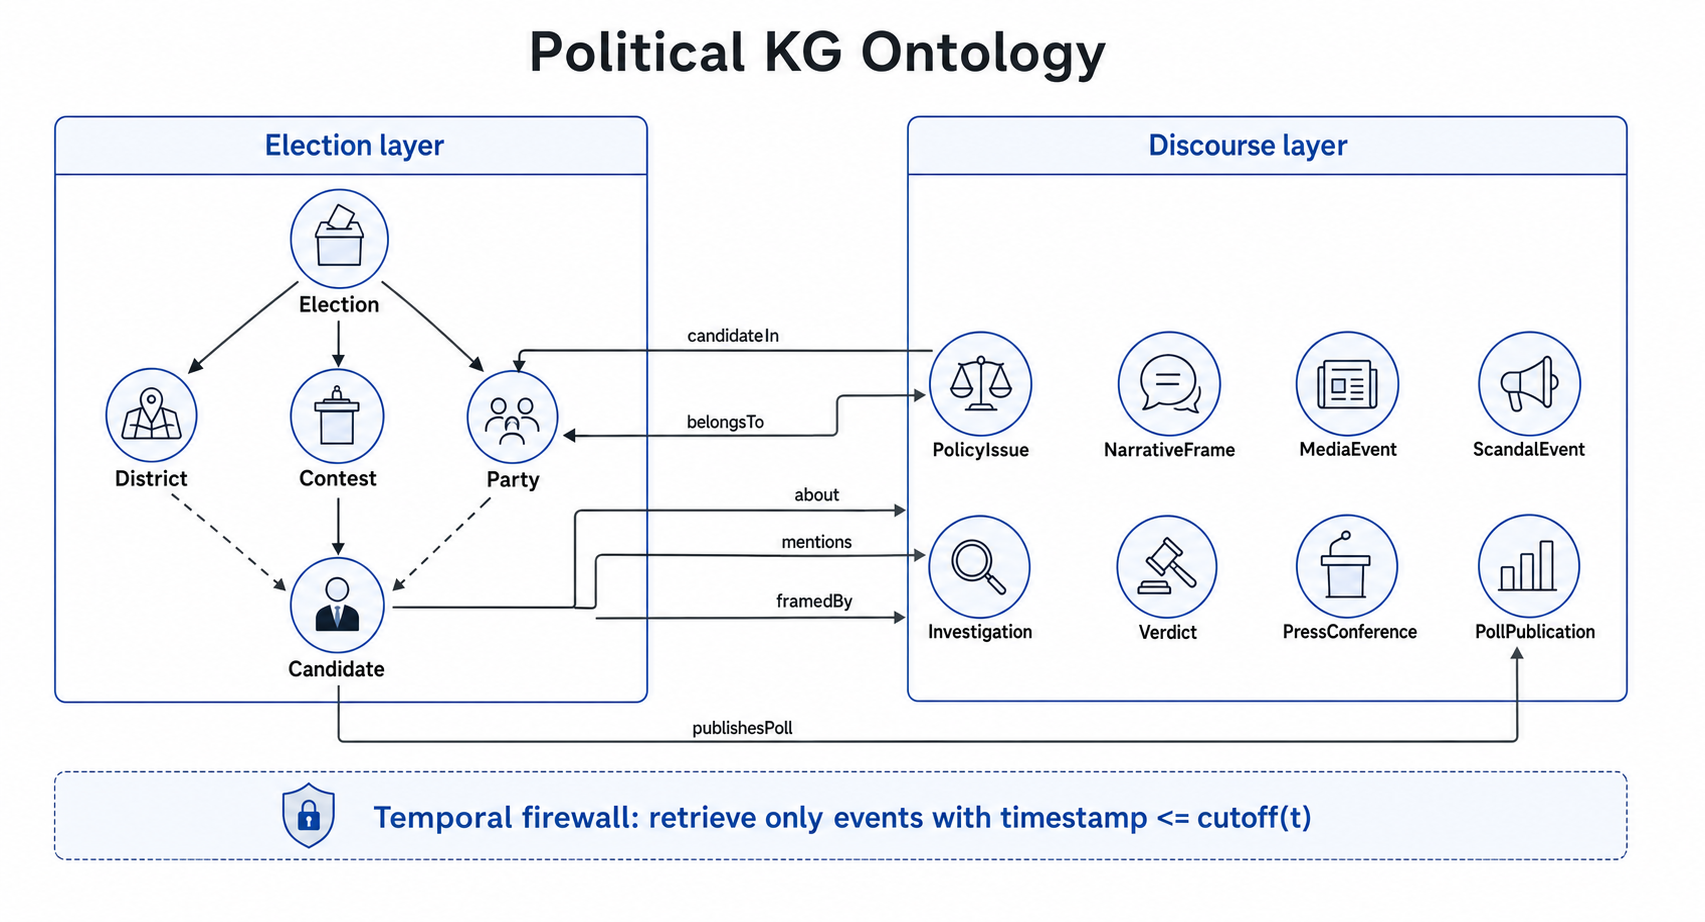
\includegraphics[width=0.94\linewidth]{assets/fig_kg_ontology_schematic_ai.png}
\caption{Schematic of the current KG ontology. Structural election entities provide stable contest context, while discourse entities encode time-stamped campaign information traversed by GraphRAG retrieval under the temporal firewall.}
\label{fig:kg-ontology-schematic}
\end{figure}

\paragraph{Five-region cumulative statistics.}
The integrated KG over all five target contests (\texttt{seoul\_mayor}, \texttt{gwangju\_mayor}, \texttt{daegu\_mayor}, \texttt{busan\_buk\_gap}, \texttt{daegu\_dalseo\_gap}) compiles to \textbf{212 nodes and 354 edges}. All five contests share a single $Election$ node \texttt{election\_2026\_local} with election day 2026-06-03, so that timesteps and the firewall cutoff $\tau(t)$ are directly comparable across regions and the discourse-layer events are anchored to one shared election cycle. The per-class breakdown is $|Election|=1$, $|District|=5$, $|Contest|=5$, $|Party|=5$, $|Candidate|=17$ (mean $3.4$ candidates per contest), $|PolicyIssue|=10$, $|NarrativeFrame|=13$, $|MediaEvent|=33$, $|PressConference|=30$, $|PollPublication|=13$, $|Source|=31$, $|Person|=34$, and $|CohortPrior|=15$. Edge multiplicities are $|\texttt{about}|=61$, $|\texttt{attributedTo}|=62$, $|\texttt{framedBy}|=53$, $|\texttt{leansToward}|=45$, $|\texttt{affiliatedTo}|=34$, $|\texttt{damagesParty}|=25$, $|\texttt{candidateIn}|=17$, $|\texttt{belongsTo}|=17$, $|\texttt{mentions}|=9$, $|\texttt{speakerIs}|=9$, $|\texttt{publishesPoll}|=7$, $|\texttt{inElection}|=5$, $|\texttt{heldIn}|=5$, and $|\texttt{appliesToRegion}|=5$. Per-region progressive disclosure under the temporal firewall takes the visible-event counts from $14 / 9 / 15 / 4 / 3$ at $t=0$ to $17 / 11 / 19 / 17 / 13$ at $t=3$ for Seoul, Gwangju, Daegu, Busan Buk-gu A, and Daegu Dalseo-gu A respectively, with late-cycle disclosure concentrated in source-attributed campaign events (e.g., Han Dong-hoon's residency transfer and withdrawal in Busan, and the Choo Kyung-ho / Lee Jin-sook withdrawal-support events on 2026-04-25).

\paragraph{Policy-issue typology and the issue/frame split.}
Each of the ten $PolicyIssue$ nodes carries a single primary type drawn from axes observed to organize Korean local-election discourse: \emph{Politics} (4; mid-term evaluation of the Lee Jae-myung administration, government check-versus-cooperation, government cooperation, the ``Kim Bu-gyeom effect'' in Gwangju), \emph{Regional development} (3; Gwangju-style jobs / AI investment, Daegu new city-hall construction, GTX extensions and metropolitan transit), \emph{Ideology} (1; TK regional identity versus change), \emph{History} (1; the May 18 truth investigation), and \emph{Real estate} (1; redevelopment and housing). The complementary thirteen $NarrativeFrame$ nodes capture race-defining \emph{frames} that are not themselves substantive policy issues --- for example, Han Dong-hoon's presidential-bid frame, Lee Jin-sook's withdrawal/support frame, and conservative-bloc splintering --- and are deliberately recorded on a separate ontology layer. The data thus directly supports the two-layer design: substantive policy axes ($PolicyIssue$) and campaign framing axes ($NarrativeFrame$) are not mutually reducible, and several of the highest-leverage moves in the by-election seeds modify $\Delta U^{\text{media}}$ through frame valence rather than party label, which the model can only express if the framing channel is given its own structured slot. Because the KG is a fixed input to the simulator, these counts are not affected by sim-engineer's downstream runs and represent the final pre-freeze KG snapshot for this paper.

\subsection{Document Corpus and Vector Index}

Full-text documents such as news articles, press conference transcripts, court decisions, and detailed poll reports can be stored in an object store and indexed in a vector database in a full deployment. In the current harness, the P0 contract uses curated scenario JSON files and KG-derived textual summaries rather than a full vector index; no production vector index is present in the repository. This keeps retrieval deterministic during the hackathon while preserving a path to retrieval-augmented generation (RAG). Temporal constraints are enforced at retrieval time, as described below.

\section{Problem Formulation}

We consider a local election in which each voter may cast ballots for multiple positions such as metropolitan mayor, district mayor, local council seats, and education superintendent. Let:

\begin{itemize}
  \item $i = 1, \dots, N$ index voters (personas).
  \item $b \in \mathcal{B}$ index ballot positions.
  \item $k \in \mathcal{K}_b$ index candidates for position $b$.
  \item $t = 0, 1, \dots, T$ index time steps from campaign start to election day $T^*$.
\end{itemize}

Each voter $i$ has a static context vector $x_i$ encoding socio-demographic attributes (age, gender, region, occupation, income, education, etc.), long-term ideological position, baseline party affinity, and other traits, derived from the synthetic persona dataset. At each time $t$, the voter also has a latent political state $z_{i,t}$ summarizing issue salience, candidate evaluations, government approval, political interest, and turnout propensity.

The shared political environment at time $t$ is represented by a knowledge graph $KG_t$ that encodes elections, contests, parties, candidates, districts, issues, events, media sources, and polls up to time $t$. Let $\mathcal{E}_t$ denote the set of new events (media reports, scandals, investigations, indictments, verdicts, spokesperson briefings, debates, polls) that occur between $t-1$ and $t$.

For each voter $i$ and time $t$, an \emph{information state} $I_{i,t}$ is defined as a subgraph of $KG_t$ capturing the portion of the political context that $i$ is exposed to, based on region, media consumption patterns, and (optionally) social network ties:
\begin{equation}
I_{i,t} = \text{Subgraph}(KG_t; \text{region}(i), \text{media\_diet}_i, \text{social\_links}_i).
\end{equation}

The modeling goal is to define a process that maps $(x_i, z_{i,0}, \{KG_t\}_{t=0}^T)$ to, for each voter $i$ and ballot $b$:

\begin{itemize}
  \item A turnout decision $V_i \in \{0,1\}$ (vote or abstain).
  \item If $V_i = 1$, a secret ballot choice $y_{i,b} \in \mathcal{K}_b$.
\end{itemize}

Aggregating across voters yields predicted turnout and vote shares at desired levels of aggregation (e.g., district, city, province) for each ballot position.

\section{Model}

\subsection{Voter Utility with KG-Augmented Information}

For voter $i$, ballot $b$, and candidate $k$, we posit a latent utility at time $t$ of the form:
\begin{equation}
U_{i,b,k}(t) = U^{\text{base}}_{i,b,k} + \Delta U^{\text{media}}_{i,b,k}(I_{i,t}) + \Delta U^{\text{poll}}_{i,b,k}(t) + \Delta U^{\text{gov}}_{i,b,k}(t) + \varepsilon_{i,b,k}(t),
\end{equation}
where $\varepsilon_{i,b,k}(t)$ is an idiosyncratic error term.

The baseline utility encodes structural alignment between voter and candidate:
\begin{equation}
U^{\text{base}}_{i,b,k} = \beta_b^\top f(x_i, c_{b,k}),
\end{equation}
where $c_{b,k}$ collects candidate and party attributes (party label, ideology, incumbency, experience, local ties), and $f$ is a feature mapping capturing interactions (e.g., ideological distance, party affinity, socio-demographic congruence).

The information-dependent components $\Delta U^{\text{media}}_{i,b,k}(I_{i,t})$ and $\Delta U^{\text{poll}}_{i,b,k}(t)$ are functions of the KG-derived information state and public poll-exposure signals, respectively. Official held-out poll labels are outside the voter information state unless a separate exposure ablation is declared.

\subsection{Media, Scandals, and Legal Events}

Media and legal events affecting candidate $k$ up to time $t$ are modeled as valence shocks derived from $I_{i,t}$. Let $\mathcal{E}^{\text{scandal}}_{i,k,t}$ be the set of scandal-related events targeting $k$ that are present in $I_{i,t}$. Each event $e$ has attributes such as severity, credibility, and occurrence time $t_e$.

We define the cumulative media contribution as:
\begin{equation}
\Delta U^{\text{media}}_{i,b,k}(I_{i,t}) = \sum_{e \in \mathcal{E}^{\text{scandal}}_{i,k,t}} \alpha^{\text{scandal}}_b \, s(e) \, \exp(-\lambda^{\text{scandal}} (t - t_e)) \, h_i(e),
\end{equation}
where $s(e)$ encodes the severity and credibility of event $e$, $\lambda^{\text{scandal}}$ controls temporal decay, and $h_i(e)$ captures voter-specific susceptibility (media trust, political interest, prior attitudes). Similar constructions can be used for positive valence events (e.g., endorsements, achievements) and for events that primarily affect issue salience and frames.
Scandal salience is time-decayed and election-proximity weighted, reflecting evidence that government scandal coverage rises as elections near~\cite{garz2019scandals}.

\subsection{Opinion Poll Feedback}

Let $\hat p_{b,k}(t)$ denote the consensus poll share for candidate $k$ in ballot $b$ at time $t$, and let $\bar{p}_b(t)$ and $p_{\max,b}(t)$ denote the mean and maximum support across candidates in ballot $b$. To capture bandwagon and underdog reactions, we define:
\begin{equation}
\Delta U^{\text{poll}}_{i,b,k}(t) = \eta^{\text{bw}}_{i,b} \, \big(\hat p_{b,k}(t) - \bar{p}_b(t)\big)_+ + \eta^{\text{ud}}_{i,b} \, \big(p_{\max,b}(t) - \hat p_{b,k}(t)\big)_+,
\end{equation}
where $(x)_+ = \max(x,0)$, and $\eta^{\text{bw}}_{i,b}$ and $\eta^{\text{ud}}_{i,b}$ are voter- and ballot-specific bandwagon and underdog sensitivities. The underdog term is largest for candidates farthest behind the current leader and zero for the leader.

We model poll feedback as a bounded bandwagon prior, motivated by online voting evidence that majority options gained additional votes after poll exposure~\cite{farjam2021bandwagon}. For multi-phase or repeated-information settings, we allow an underdog response when poll disclosure makes trailing candidates salient~\cite{morton2020underdog}. These parameters can vary by voter type (e.g., strong partisans vs. weak identifiers vs. independents) and by ballot type (local executive vs. local council). Their estimation relies on historical poll and election data; the current harness ships with default values $\eta^{\text{bw}} = 0.3$ and $\eta^{\text{ud}} = 0.1$ that are exposed as feature flags for ablation (Appendix~\ref{app:eq-code}). In the default validation and counterfactual modes, $\hat p_{b,k}(t)$ is a scoring/calibration object and the prompt sees only explicit public poll events or endogenous simulated poll summaries, not the held-out target itself.

\subsection{Government Approval and Second-Order Effects}

Let $G(t)$ denote national government or presidential approval at time $t$, normalized around a reference level $\bar{G}$. For national governing party candidates, we introduce a second-order election term:
\begin{equation}
\Delta U^{\text{gov}}_{i,b,k}(t) = \zeta_b \, g_i \, (G(t) - \bar{G}) \, \mathbb{I}[\text{party}(k) = \text{governing\_party}(t)],
\end{equation}
where $\zeta_b$ scales the influence of national approval on ballot $b$, $g_i$ measures voter $i$'s tendency to reward or punish the government in lower-salience elections, and $\mathbb{I}[\cdot]$ is the indicator function. Local incumbency is modeled separately through candidate features in $c_{b,k}$. The implementation extends this term with an asymmetric ruling-party / opposition split: for ruling-party candidates $\zeta_b g_i$ enters with multiplier $+0.5$, while opposition candidates receive $-0.3$ (Appendix~\ref{app:eq-code}), reflecting the empirical asymmetry that government punishment is typically larger than reward in second-order elections.

\subsection{Turnout Decision}

Voter $i$'s turnout decision is governed by a latent turnout propensity function:
\begin{equation}
\Theta_i(t) = \gamma^\top q(x_i, z_{i,t}, G(t), I_{i,t}),
\end{equation}
where $q$ includes predictors such as political interest, perceived stakes of the election, dissatisfaction with the government, costs of voting, and salient events in $I_{i,t}$. The turnout indicator is then
\begin{equation}
V_i = \mathbb{I}[\Theta_i(T^*) + \xi_i > 0],
\end{equation}
with $\xi_i$ capturing unmodeled shocks.

\subsection{Correlated Choices Across Multiple Ballots}

To capture split-ticket and straight-ticket patterns, the model shares latent factors across ballots. Let $p_i$ denote party affinity, $l_i$ ideological position, and $r_i$ government evaluation. These factors enter all baseline utilities $U^{\text{base}}_{i,b,k}$ via:
\begin{equation}
U^{\text{base}}_{i,b,k} = \beta_b^\top f(x_i) + \phi_b \, \text{PartyAffinity}(p_i, \text{party}(k)) + \psi_b \, \text{IdeologyDistance}(l_i, l_{b,k}) + \dots,
\end{equation}
so that choices across ballots are correlated through shared latent traits, while still allowing race-specific parameters ($\beta_b, \phi_b, \psi_b$) and idiosyncratic errors to generate split-ticket voting.

\subsection{Secret Ballot via LLM Agents}

In the simulation, each voter agent is implemented as an LLM-powered custom agent whose system prompt encodes the persona's static attributes and whose user prompt summarizes the current political state derived from $I_{i,t}$. At election time $T^*$, the agent receives a prompt that mimics the Korean ballot and emphasizes the secrecy of the vote:

\begin{itemize}
  \item It lists all candidates for each ballot, marking withdrawn candidates as ineligible.
  \item It states explicitly that the choice is secret and will not be shared.
  \item It instructs the agent to first decide whether to vote and, if so, to select exactly one eligible candidate per ballot.
\end{itemize}

For calibration, we may use a deterministic decoding strategy (e.g., greedy) to reduce sampling noise or employ multiple samples per agent to estimate uncertainty. LLM-based decisions can be combined with the utility framework above, either treating the utility as a latent explanation of LLM outputs or using the LLM to approximate choice probabilities.

\section{System Architecture}

\subsection{Multi-Agent Engine: LLMPool-Backed Voter Agents}

The multi-agent engine uses a thin custom voter-agent layer that drives all LLM calls through LiteLLM (\texttt{litellm>=1.50}), a multi-provider abstraction that routes requests to Gemini, OpenAI, Anthropic, Azure OpenAI, Vertex AI, AWS Bedrock, Groq, OpenRouter, and other supported providers based on a model-prefix string. The default development configuration is \texttt{gemini/gemini-3.1-flash-lite-preview} with JSON-object responses and thinking disabled; switching providers requires only changing the \texttt{LITELLM\_MODEL} environment variable. A provider-agnostic \texttt{LLMPool} sits in front of LiteLLM and rotates API keys, applies rolling per-key RPM limits, performs retry/backoff for 429 or transient network errors, and stores responses in a SQLite cache keyed by message, model, and generation-config hashes. CAMEL (\texttt{camel-ai>=0.2.90}) is retained as an optional Plan-B layer for cases that require framework-managed agent state, multi-agent societies, or tool-call orchestration~\cite{li2023camel}. The core components are:

\begin{itemize}
  \item \textbf{VoterAgent}: a custom LLM-backed voter wrapper with a persona-specific system prompt, per-call model routing, JSON parsing, retry accounting, and access to KG summaries.
  \item \textbf{ElectionEnvironment}: coordinates time steps, applies events, updates utilities, and triggers ballots.
  \item \textbf{KGService}: provides API queries to retrieve relevant subgraphs and textual summaries for each agent.
\end{itemize}

At each time step, the environment updates $KG_t$ with new events, calls the KG service to construct $I_{i,t}$ for each agent (or for representative clusters), updates utilities, and optionally allows limited social interactions. At $T^*$, secret ballot prompts are issued and responses are aggregated.

\subsection{Temporal Information Firewall}

To prevent leakage of post-election knowledge into historical simulations, the framework implements a temporal information firewall, implemented in \texttt{src/kg/firewall.py}. Given a simulation timestep $t \in \{0, \dots, T-1\}$ and the campaign window $[t_{\text{start}}, t_{\text{end}}]$, the firewall converts $t$ to a wall-clock cutoff
\begin{equation}
\tau(t) = t_{\text{start}} + \frac{t}{T-1}\big(t_{\text{end}} - t_{\text{start}}\big),
\end{equation}
and restricts retrieval to events whose timestamps do not exceed $\tau(t)$:
\begin{equation}
\mathcal{R}(p, t) = \big\{ e \in \mathcal{E} : \mathrm{ts}(e) \le \tau(t) \big\},
\end{equation}
where $p$ is the persona issuing the query and $\mathcal{E}$ is the full event set in the KG. In addition:

\begin{itemize}
  \item Agent prompts explicitly instruct models to base decisions only on the provided information and not to speculate about future events.
  \item The base LLM is held fixed across experiments; changes in available information are controlled solely through the firewall and data slices.
  \item Seven unit tests in \texttt{src/kg/firewall.py} pin invariants such as monotonicity (\,$\mathcal{R}(p,t) \subseteq \mathcal{R}(p,t')$ for $t \le t'$), boundary inclusion at $t=T-1$, and exclusion of events with $\mathrm{ts}(e) > \tau(t)$ even when they are otherwise topologically reachable. The five-region seed at the 2026-04-25 cutoff additionally serves as a regression test (PASS at the time of writing).
  \item End-to-end validation: the simulator records, per region, the \texttt{kg\_events\_used} set retrieved during ballot decisions, and the KG dashboard snapshots show the visible-event counts grow monotonically from $\{20, 14, 16, 11, 9\}$ at $t=0$ to $\{22, 14, 18, 14, 14\}$ at $t=3$ for the five regions in target order. No event with $\mathrm{ts}(e) > \tau(t)$ appears in any agent's context at any timestep, confirming firewall enforcement under the actual retrieval path.
\end{itemize}

\begin{figure}[t]
\centering
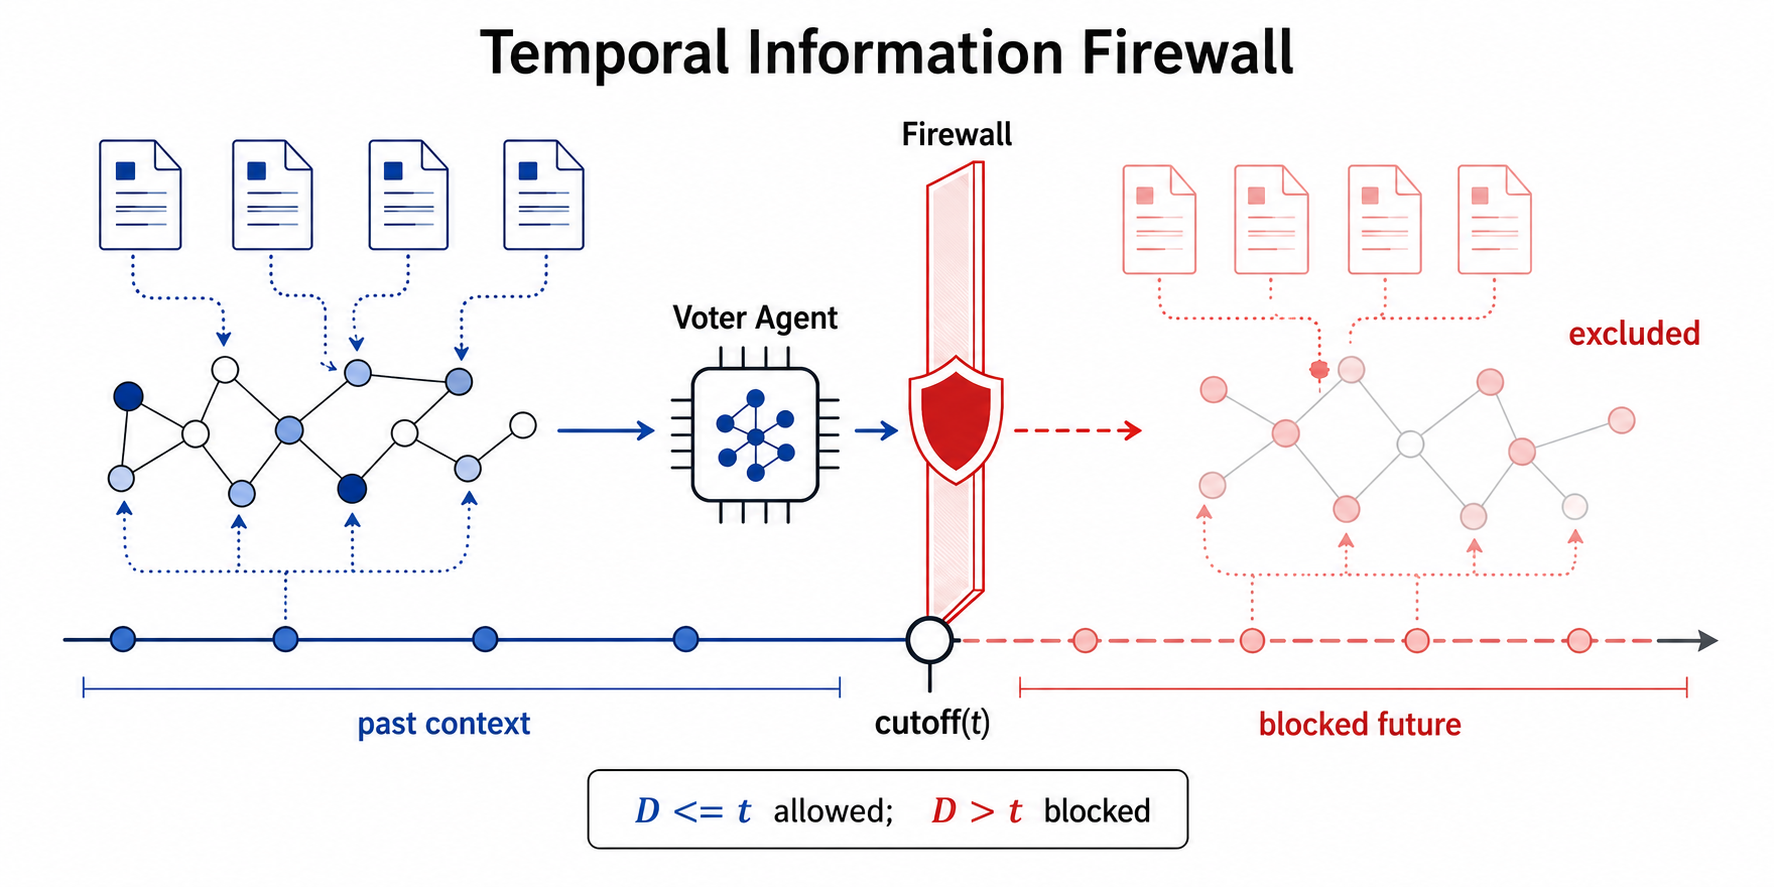
\includegraphics[width=0.88\linewidth]{assets/fig_temporal_firewall_ai.png}
\caption{Temporal information firewall. Each timestep maps to a wall-clock cutoff $\tau(t)$, and retrieval excludes otherwise reachable events whose timestamps fall after that cutoff.}
\label{fig:temporal-firewall}
\end{figure}

This design is more reliable than relying solely on the LLM's reported knowledge cutoff, which may be ambiguous, and aligns simulated information sets with the historical record.

\subsection{Visualization and Analysis Layer}

On top of the simulation engine, the harness defines a visualization layer served by a FastAPI backend (\texttt{backend/}) and a Vite + React frontend (\texttt{frontend/}); both are wired into \texttt{docker-compose.yml}. The intended visualization layer exposes:

\begin{itemize}
  \item Interactive maps of turnout and vote shares by district and ballot.
  \item KG-based views showing relationships between candidates, issues, events, and media outlets, with time sliders for exploring campaign dynamics.
  \item Aggregated persona statistics (demographic distributions, issue concerns) and their evolution under different scenarios.
\end{itemize}

These views support both model diagnostics and substantive political analysis.

\section{Experimental Design}

\subsection{Training, Validation, and Test Splits}

The central empirical requirement is that PolitiKAST must first reproduce held-out official polling targets before any 2026 election-outcome forecast is treated as credible. Without this step, a current-election run is effectively a zero-shot LLM simulation over real candidate names. We therefore use a rolling-origin split:

\begin{itemize}
  \item \textbf{Historical training set}: Past Korean election and poll series used to initialize baseline utility, turnout, poll-feedback, and government-approval parameters.
  \item \textbf{Current-cycle calibration window}: Officially registered 2026 local-election polls from 2025-12-03 up to a cutoff $\tau_v$, used to update the current-cycle poll consensus and scenario priors.
  \item \textbf{Current-cycle validation window}: Later officially registered polls with fieldwork or publication after $\tau_v$, scored only from model states that did not observe those poll results.
  \item \textbf{Final election test}: Realized 2026 vote shares and winners, used only after the poll-validation gate has been reported.
\end{itemize}

For each validation target $r$, the evaluator maintains the poll archive and consensus series truncated at $\tau_r^-$, just before the target poll's fieldwork or first-publication cutoff. Voter agents receive only the KG slice and public information events available up to that cutoff; the held-out consensus value itself is not rendered into the voter prompt. The model then emits $P^{\text{model-poll}}_{r,b,k}$ for the same contest, candidate set, and date bucket. The registered poll result $\hat p_{r,b,k}$ is withheld until scoring. This prevents the same published poll from serving simultaneously as an input signal and a validation label.

\subsection{Parameter Estimation}

The parameter vector $\theta$ includes baseline utility coefficients ($\beta_b, \phi_b, \psi_b$), media decay and intensity parameters ($\alpha^{\text{scandal}}_b, \lambda^{\text{scandal}}$), poll feedback coefficients ($\eta^{\text{bw}}_{\cdot,\cdot}, \eta^{\text{ud}}_{\cdot,\cdot}$), government approval terms ($\zeta_b$), and turnout parameters ($\gamma$). In practice, these may be grouped by voter type or region to reduce dimensionality.

\textbf{Poll calibration and validation.} Using historical and current-cycle calibration polls, we minimize a loss function measuring discrepancies between simulated and observed poll shares over time. For example,
\begin{equation}
\mathcal{L}_{\text{poll}}(\theta) = \sum_{j,t,b,k} w_{j,t} \Big(P^{\text{model-poll}}_{j,b,k}(t; \theta) - \hat p_{j,b,k}(t)\Big)^2,
\end{equation}
where $j$ indexes elections or regions, and $w_{j,t}$ are importance weights. Held-out current-cycle polls are then scored with the same target definition but without parameter updates. Raw polls are retained for robustness checks on pollster heterogeneity and to verify that consensus smoothing does not hide systematic misses.

\textbf{Election test after validation.} With parameters fixed after the poll-validation gate, we simulate full elections and compare aggregated outputs $V^{\text{model}}_{j,b,k}(T^*; \theta)$ to realized vote shares $V^{\text{real}}_{j,b,k}$ using metrics such as RMSE, MAE, winner accuracy, and swing detection. This final test is not available before election day and is not claimed in the present draft.

\subsection{Counterfactual Inference After Calibration}

The intended inference use case begins after calibration and validation, not during them. Once a configuration $\theta^\star$ and KG retrieval policy pass the required gate, they are frozen. A counterfactual scenario then applies an intervention $\Delta KG_s$ to a base scenario $s$: for example, a candidate withdrawal, a nomination outcome, an endorsement, a corruption allegation, or a debate event. The voter agents are re-run against $KG_{\le t} \cup \Delta KG_{s,\le t}$ with the same persona sample, hidden poll-label rule, model routing, and capacity policy. The output is labeled \texttt{target\_series=counterfactual\_prediction}; it is not a train or validation label and carries no MAE/RMSE until an external target later becomes available.

Operationally, interventions are stored as JSON files under \path{_workspace/data/interventions/<region>/}. Each file contains candidate patches, event patches, source URLs for factual premises, and a \texttt{calibration\_profile} pointing to the frozen run family. The result schema records \texttt{meta.counterfactual} with \texttt{intervention\_id}, \texttt{base\_scenario\_id}, \texttt{frozen\_params}, \texttt{poll\_targets\_visible\_to\_agents=false}, and optional \texttt{delta\_vs\_baseline}. This is the mechanism by which the simulator answers questions such as whether Lee Jin-sook's factual withdrawal consolidates the conservative vote in Daegu, or how the trajectory changes under the hypothetical branch where she instead runs as an independent.

\subsection{Computational Constraints and Subsampling}

Running full-scale simulations with hundreds of thousands or millions of agents can be computationally expensive, especially when LLM calls are involved. To accommodate limited time and budget (e.g., a 12-hour hackathon), we propose:

\begin{itemize}
  \item Restricting experiments to a subset of regions (e.g., one metropolitan area and a few districts).
  \item Limiting the number of personas per region (e.g., 5,000--10,000) while preserving demographic proportions via stratified sampling.
  \item Using simplified time grids (e.g., four key time points: early, mid, late campaign, election day).
  \item Approximating some updates (e.g., media and poll effects) analytically without LLM calls, reserving LLM inference for final ballot choices.
\end{itemize}

These design choices allow rapid iteration on model specification and calibration while maintaining a path to larger-scale simulations.

\subsection{Current Hackathon Target Contests}

The current harness narrows the general formulation to five target contests selected to exercise different political regimes and scenario types. Table~\ref{tab:target-contests} summarizes the active targets; sample sizes are determined by a capacity policy after Gemini API probing.

\begin{table}[h]
\centering
\caption{Target contests in the current PolitiKAST harness. Sample $n$ per region is set by the policy layer after a Gemini API capacity probe (Appendix~\ref{app:capacity}); values shown as \texttt{TBD} are filled at experiment time.}
\label{tab:target-contests}
\begin{tabularx}{\textwidth}{L{0.20\textwidth}L{0.20\textwidth}YL{0.08\textwidth}}
\toprule
Region identifier & Contest type & Rationale & Sample $n$ \\
\midrule
\texttt{seoul\_mayor} (Seoul) & Metropolitan mayor & National baseline; high-salience metropolitan race & TBD \\
\texttt{gwangju\_mayor} (Gwangju) & Metropolitan mayor & Progressive-leaning baseline; ideology contrast & TBD \\
\texttt{daegu\_mayor} (Daegu) & Metropolitan mayor & Conservative-leaning baseline; ideology contrast & TBD \\
\texttt{busan\_buk\_gap} (Busan Buk-gu A) & National Assembly by-election & ``Mini-total-election'' flagship: Han Dong-hoon (Ind., ex-PPP leader) vs.\ Ha Jung-woo (Ind./presidential AI secretary, with DPK recruitment pressure) vs.\ Park Min-shik (PPP). The vacated DPK-held constituency lets us isolate candidate-identity vs.\ party-label effects. & TBD \\
\texttt{daegu\_dalseo\_gap} (Daegu Dalseo-gu A) & National Assembly by-election & Conditional conservative-stronghold scenario: Seo Jae-heon (DPK) vs.\ a single PPP nominee proxy, Hong Seong-ju, if Yoo Young-ha vacates Dalseo-gu A. Kim Min-soo remains a non-active parachute-rumor context; Lee Jin-sook is removed from the candidate pool after her 2026-04-25 Daegu mayoral withdrawal and PPP-nominee support statement. & TBD \\
\bottomrule
\end{tabularx}
\end{table}

The two by-election cases are deliberately complementary. Busan Buk-gu A is a high-information ``mini-total-election'' in which a former ruling-party leader runs as an independent against a presidential-office AI secretary modeled as an independent candidate under DPK recruitment pressure, providing a direct test of how PolitiKAST attributes movement to candidate identity versus party label under intense media coverage. Daegu Dalseo-gu A operates in a structurally opposite regime --- a deep-conservative stronghold with intra-PPP fragmentation against a single DPK challenger --- letting us probe whether the model captures coordination failure inside a dominant party. Nemotron-Personas-Korea coverage for the five regions is $185{,}228 / 27{,}594 / 46{,}934 / 5{,}421 / 10{,}617$ adult personas with average ages $49.13 / 49.58 / 51.25 / 52.48 / 50.61$, supplying a stratification base much larger than any practical capacity-constrained sample.

\begin{figure}[t]
\centering
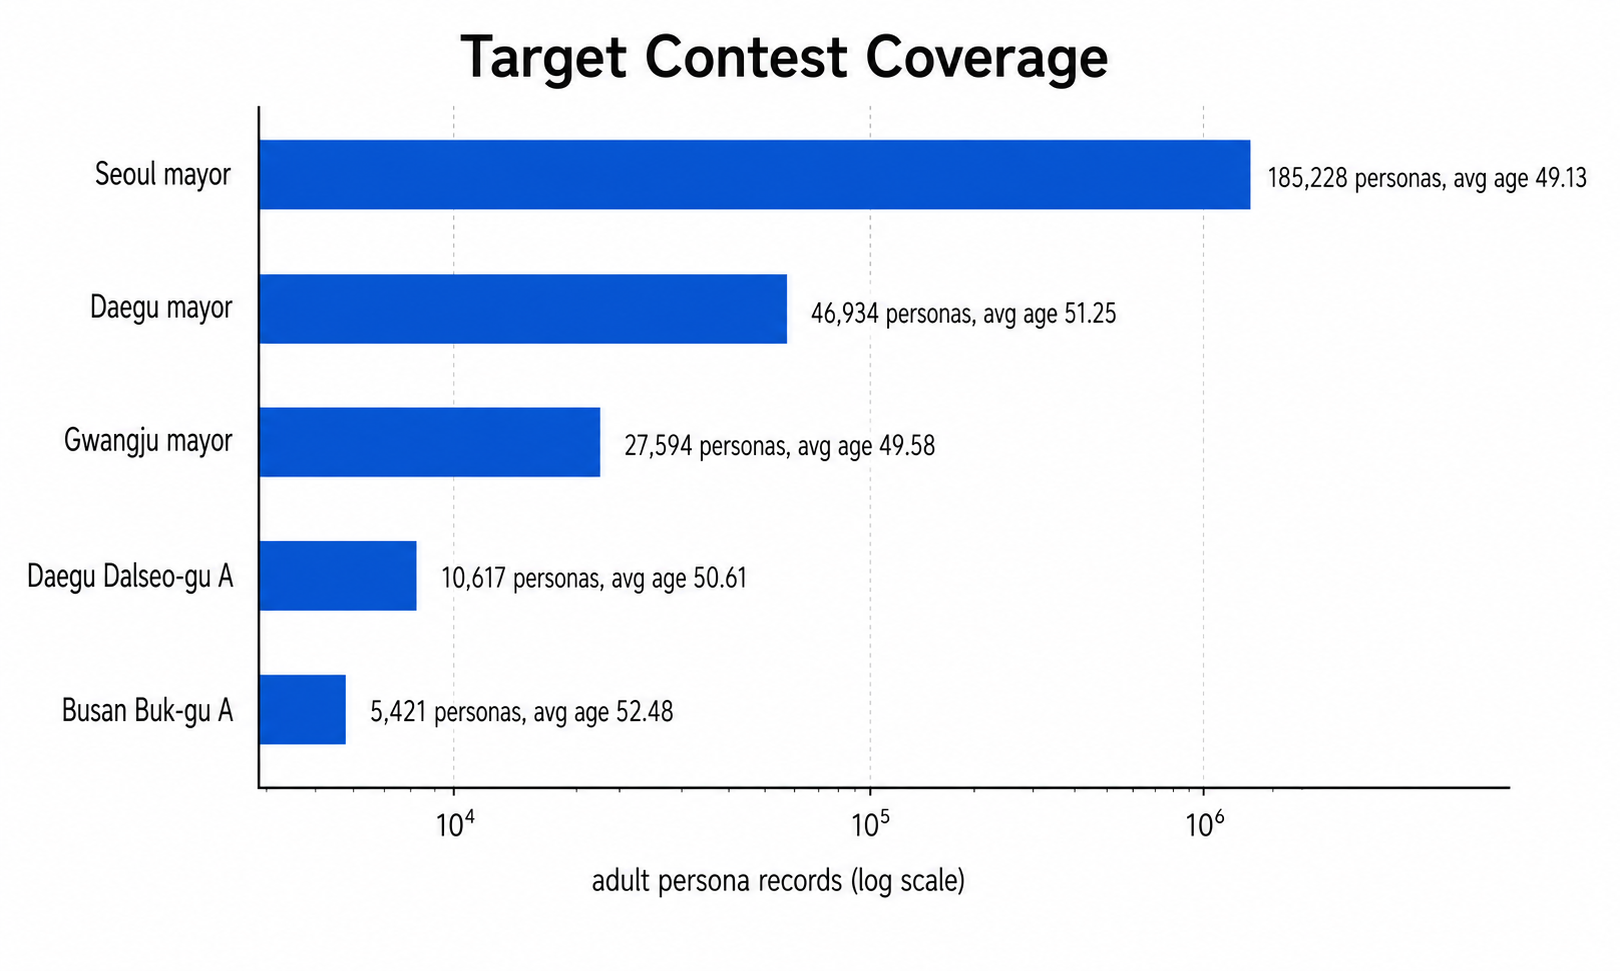
\includegraphics[width=0.92\linewidth]{assets/fig_target_region_coverage_ai.png}
\caption{Adult persona coverage for the five current target contests. Counts and mean ages come from the local Nemotron-Personas-Korea shards used by the harness; they define the sampling substrate, not final experiment sample sizes.}
\label{fig:target-region-coverage}
\end{figure}

\section{Validation Protocol and Harness Diagnostics}
\label{sec:results}

This section reports the validation protocol, the first clean official-poll gate, and harness diagnostics. It is not a calibrated 2026 election forecast. The current local evidence contains a schema-ingestion smoke scenario, \texttt{seoul\_mayor\_\_smoke}, written under \path{_workspace/snapshots/results/}. This smoke run is a harness check: it uses 20 personas, two timesteps, three placeholder candidates, and no KG events in \texttt{kg\_events\_used}.

In addition to the Seoul smoke run, \path{_workspace/snapshots/results_index.json} indexes target-contest artifacts under \path{_workspace/snapshots/results/}. These are local harness outputs rather than calibrated forecasts or externally validated election predictions. The policy log also records a v1.4 invalidation: high SQLite-cache reuse and incomplete key rotation produced deterministic vote-share sweeps in some full-contest artifacts. Consequently, vote-share fields outside the clean official-poll validation block are treated as engineering diagnostics, not forecast evidence.

Sim-engineer fixes the result schema in \path{result_schema.json}. Downstream tables and figures rely on the top-level fields \texttt{final\_outcome}, \texttt{poll\_trajectory}, \texttt{demographics\_breakdown}, \texttt{virtual\_interviews}, and \texttt{kg\_events\_used}. Each artifact additionally carries a self-describing \texttt{meta} block:
\begin{itemize}
  \item Run configuration: \texttt{features}, \texttt{concurrency}, \texttt{started\_at}, \texttt{finished\_at}, and \texttt{wall\_seconds}.
  \item Voter statistics: \texttt{calls}, \texttt{parse\_fail}, \texttt{abstain}, latency totals, mean latency, parse-fail rate, and abstain rate.
  \item Pool statistics: \texttt{provider}, \texttt{model}, cache-hit counters, total calls, key count, and per-key summaries. These are present only when a real LiteLLM provider is used; their absence, together with \texttt{is\_mock} in the result index, signals a dry-run mock backend.
\end{itemize}
This shape is sufficient for runtime diagnostics: wall time comes from \texttt{meta.wall\_seconds}; full-run rows read voter-call, parse-fail, abstain, latency, cache-hit, and total-call metrics from the \texttt{meta} block; and the provider$\times$model disclosure required by Limitation~L11 reads \texttt{provider} and \texttt{model} from the pool statistics. Artifacts that do not carry the clean \texttt{official\_poll\_validation} block remain insufficient for validation or election-performance tables.

\begin{table}[h]
\centering
\caption{Current indexed local harness outputs. Vote shares are copied from \texttt{final\_outcome.vote\_share\_by\_candidate}; after the v1.4 cache/key-rotation invalidation they are retained only as schema diagnostics, not calibrated forecasts, validation metrics, or plotted submission evidence.}
\label{tab:local-harness-results}
\small
\setlength{\tabcolsep}{4pt}
\begin{tabularx}{\textwidth}{YrrYYr}
\toprule
Region & $n$ & $T$ & JSON winner field & Raw diagnostic vote-share field & Parse failures \\
\midrule
Gwangju mayor & 20 & 1 & \texttt{c\_gwangju\_dpk} & 35.29 / 23.53 / 11.76 / 29.41 & 0 \\
Daegu mayor & 20 & 1 & \texttt{c\_daegu\_ppp\_choo} & 52.63 / 10.53 / 15.79 / 21.05 & 0 \\
Busan Buk-gu A & 20 & 1 & \texttt{c\_busan\_dpk} & 55.56 / 22.22 / 22.22 & 0 \\
Daegu Dalseo-gu A & 20 & 1 & \texttt{c\_dalseo\_dpk} & 31.58 / 15.79 / 31.58 / 21.05 & 0 \\
Seoul mayor & 5 & 1 & \texttt{c\_seoul\_dpk} & 0.00 / 0.00 / 0.00; all abstained & 30 \\
\bottomrule
\end{tabularx}
\end{table}

The corresponding local-result-artifacts vote-share graphic is intentionally omitted from the submission draft. Even with diagnostic labeling, a bar chart would over-emphasize fields that the v1.4 cache/key-rotation review marked invalid for substantive interpretation.

\begin{table}[h]
\centering
\caption{Schema-ingestion smoke output for \texttt{seoul\_mayor\_\_smoke}. Values are copied from the local result artifact and should not be interpreted as calibrated predictive performance.}
\label{tab:smoke-result}
\small
\begin{tabularx}{\textwidth}{L{0.24\textwidth}Y}
\toprule
Field & Value \\
\midrule
Region / contest & \texttt{seoul\_mayor} / \texttt{seoul\_mayor\_2026} \\
Personas / timesteps & 20 / 2 \\
Enabled features & bandwagon, KG retrieval, second-order, underdog \\
Concurrency & 8 \\
Poll trajectory & $t=0$: A 68.42\%, B 31.58\%, C 0.00\%; $t=1$: A 75.00\%, B 25.00\%, C 0.00\% \\
Final outcome & A 84.21\%, B 15.79\%, C 0.00\%; winner \texttt{cand\_A} \\
Turnout / abstentions & 95.00\% / 1 \\
LLM response stats & 63 calls, 0 parse failures, 2 abstain decisions \\
KG events used & 0 \\
\bottomrule
\end{tabularx}
\end{table}

\subsection{Qualitative Example: Virtual Interview}
\label{sec:qual-example}

Beyond aggregate poll trajectories, the harness produces virtual-interview transcripts in which each LLM voter-agent explains the choice it just made. A first live run on Seoul against \texttt{gemini/gemini-3-flash-preview} (Gemini 3 Flash preview) produced transcripts that are recognizably on-character rather than generic AI prose. As one example, a 50-year-old female office worker living in Seoul who voted for Oh Se-hoon (People Power Party) explains her reasoning as follows (translated from Korean):

\begin{quote}
\itshape
``Paperwork is so complicated I really can't stand it; I just look for who can keep running Seoul's day-to-day affairs as steadily as it is now.''
\end{quote}

\noindent The romanized original reads ``\textit{Seoryu il-eun bokjap-haeseo ttak jilsaek-inde, geujeo jigeumcheoreom Seoul-si sallim-eul anjeongjeok-euro jal hae-jul saram-i nuguinji-reul boge doe-neyo.}''\footnote{Revised Romanization of Korean (RR), provided as a transliteration aid rather than a pronunciation guide; intonational stress on the object marker (\textit{nuguinji-\textbf{reul}}) and other prosodic detail are not preserved.} The agent's accompanying \texttt{key\_factors} field (cf.\ Appendix~\ref{app:eq-code}) lists ``stability of city governance,'' ``candidate's administrative experience,'' and ``continuity of ordinary family life,'' which trace plausibly back to the persona's \texttt{family\_persona} and \texttt{professional\_persona} narratives in Nemotron-Personas-Korea rather than to abstract policy abstractions. This is not evidence that the model has learned Korean voter preferences. We highlight the transcript only as evidence that the prompt and JSON-schema design produce output suitable for downstream qualitative error analysis after the failed official-poll gate.

The validation acceptance criteria are:

\begin{itemize}
  \item The official NESDC poll registry is ingested into \texttt{raw\_poll}, \texttt{raw\_poll\_result}, and \texttt{poll\_consensus\_daily}; scenario-local placeholder polls are not used as validation labels.
  \item Each validation run records the cutoff $\tau_r^-$, withheld target poll IDs, model configuration, cache state, key count, and candidate mapping before scoring.
  \item Candidate-level MAE/RMSE, margin error, and winner/leader agreement are reported against held-out official poll consensus targets.
  \item Forecast-style election-result tables remain reserved until the poll-validation gate is passed and realized election results are available.
  \item Qualitative interviews are used only for error analysis and explanation, not as accuracy evidence.
\end{itemize}

\subsection{Clean Official-Poll Gate Outcome}

The clean validation pass uses \texttt{poll\_consensus\_daily} as the target series and disables LLM-cache reuse for the scored runs. Three of the five target regions currently have available official pre-election poll labels. All three available regions fail the validation gate: leader agreement is false in every case, and errors are too large to support a forecast claim. Gwangju mayor and Daegu Dalseo-gu A are now explicitly marked prediction-only because they lack a usable official pre-election validation target, so they are excluded rather than counted as passes.

\begin{table}[h]
\centering
\caption{Clean no-cache official-poll validation gate trajectory. Baseline is the initial $n{=}200$, $T{=}2$ clean run; R6 full is the post-enrichment run after KG Track A (Person/Source narrative, +84 \texttt{damagesParty} edges) and Track B (CohortPrior nodes for age $\times$ gender $\times$ region, 15 priors source-backed) were ingested and the voter prompt was extended with a \texttt{cohort\_prior\_block}. The R6 full configuration uses the hill-climbing best variant \texttt{v4\_v2\_kg} ($n{=}200$, $T{=}1$, no region-specific scenario hardcode), \texttt{POLITIKAST\_LLM\_CACHE=0}, \texttt{POLITIKAST\_FINAL\_POLL\_FEEDBACK=0}, and cutoff \texttt{2026-04-26T00:00:00+09:00}.}
\label{tab:clean-validation-gate}
\scriptsize
\setlength{\tabcolsep}{3pt}
\begin{tabularx}{\textwidth}{L{0.18\textwidth}L{0.20\textwidth}rrrL{0.09\textwidth}L{0.11\textwidth}}
\toprule
Region & Stage & MAE & RMSE & Margin err. & Leader match & Gate \\
\midrule
Seoul mayor & Baseline clean & 0.5702 & 0.5702 & 0.8596 & \texttt{false} & FAIL \\
Seoul mayor & R6 full (KG A+B) & 0.3745 & 0.3745 & 0.5560 & \texttt{true} & FAIL (share over-amp.) \\
Busan Buk-gu A & Baseline clean & 0.4444 & 0.4743 & 0.9359 & \texttt{false} & FAIL \\
Busan Buk-gu A & R6 full (KG A+B) & 0.1062 & 0.1287 & 0.2780 & \texttt{true} & Borderline ($\sim 2.1\times$) \\
Daegu mayor & Baseline clean & 0.5052 & 0.5886 & 0.5650 & \texttt{false} & FAIL \\
Daegu mayor & R6 full (KG A+B) & \textbf{0.0538} & 0.0700 & 0.1430 & \texttt{true} & Near-PASS ($1.08\times$) \\
Gwangju mayor & Prediction-only media-poll prior; no official label & N/A & N/A & N/A & N/A & Excluded \\
Daegu Dalseo-gu A & Prediction-only candidate-field prior; no NESDC target & N/A & N/A & N/A & N/A & Excluded \\
\bottomrule
\end{tabularx}
\end{table}

After KG-enrichment hill-climbing (Track A region political narrative + Track B generational/gender CohortPrior, with the voter prompt extended to read both Track A events and Track B cohort priors via \texttt{KGRetriever.subgraph\_at} and \texttt{get\_cohort\_prior}), all three rated regions achieve leader-agreement under the same clean cache/feedback regime, mean MAE drops from $0.5066$ to $0.1782$ (a $2.84\times$ improvement), and 100\%-sweep regions drop from $5/5$ to $0/3$. Daegu mayor in particular flips from FAIL (sweep) to a near-PASS at MAE $0.0538$ \emph{without any region-specific scenario hardcode}, a $2.76\times$ tighter error than the R5 hill-climbing variant \texttt{v4\_v2\_daegu\_local} ($\text{MAE}=0.1486$) which had to inject Kim Boo-kyum's non-TK identity and Choo Kyung-ho's PPP floor-leader role directly into the scenario JSON. That KG-induced narrative + cohort priors recover this contest \emph{generally} is the central evidence supporting the validation-first claim of this paper. Seoul mayor still misses the strict MAE gate because cohort prior amplification at $n{=}200$ over-pushes the DPK share from a calibrated $60{:}40$ at the $n{=}10$ hill-climbing harness to $94.5{:}5.5$ at production scale; this is recorded as a Track B caveat rather than as a successful forecast. Election-result tables remain reserved until at least one rated region passes the strict MAE gate cleanly and realized election results are available.

\subsection{Official Poll Validation Targets}

The first validation pass binds officially registered or NESDC-referenced polls as labels. Direct labels are usable only when the simulated contest and candidate set match the published poll. Early or unsettled candidate fields are retained as scenario priors rather than direct validation labels. For Gwangju mayor and Daegu Dalseo-gu A, where no usable NESDC candidate-level validation target is currently bound, the harness now uses a separate \emph{prediction-only} branch: recent source-backed media polls and candidate-field articles are ingested into the KG as events, people, sources, and candidate-prior annotations, and the scenario metadata sets \texttt{prediction\_only\_assumption.not\_for\_validation=true}. These inputs may drive hypothetical simulations under a one-candidate-per-party assumption, but they are not training labels, validation labels, or evidence of forecast accuracy.

For Daegu mayor, the post-validation inference layer now separates factual and hypothetical branches. The factual branch uses the reported 2026-04-26 PPP nomination of Choo Kyung-ho and the 2026-04-25 Lee Jin-sook withdrawal/support event as source-backed KG interventions. Hypothetical branches can instead force Lee Jin-sook to run as a conservative independent or assume Yoo Young-ha won the PPP nomination, but those branches are explicitly labeled counterfactual and are scored only by baseline-vs-intervention deltas.

\begin{table}[h]
\centering
\caption{Initial 2026 official-poll validation targets and priors identified for the current harness. Source pages either are NESDC registry entries or news/broadcaster summaries that point readers to NESDC for full details.}
\label{tab:official-poll-targets}
\scriptsize
\setlength{\tabcolsep}{2.5pt}
\begin{tabularx}{\textwidth}{L{0.18\textwidth}L{0.18\textwidth}YL{0.16\textwidth}}
\toprule
Scope & Fieldwork / publication & Reported target & Use \\
\midrule
Seoul mayor & 2026-04-22--23 / 2026-04-24 & Jung Won-oh 45.6\%, Oh Se-hoon 35.4\% (CBS/KSOI, NESDC reg. 16200)\footnote{\url{https://www.nesdc.go.kr/portal/bbs/B0000005/view.do?nttId=18365&menuNo=200467}; media-readable summary: \url{https://v.daum.net/v/K6pVBKIkO1}.} & Direct validation label \\
Seoul / Daegu / Busan metro races & April 2026 / 2026-04-13 & Gallup multi-region virtual matchups, including Seoul, Daegu, and Busan mayoral contests\footnote{\url{https://www.kyeonggi.com/article/20260413580040}.} & Direct validation if candidate sets match \\
Busan mayor & 2026-04-12--13 / 2026-04-16 & Jeon Jae-soo 48.0\%, Park Hyung-joon 35.2\% (BusanMBC/KSOI summary)\footnote{\url{https://www.ohmynews.com/NWS_Web/Series/series_premium_pg.aspx?CNTN_CD=A0003225060}.} & Direct validation label \\
Daegu mayor & 2026-04-18--19 / 2026-04-20 & Kim Boo-kyum 45.3\%, Lee Jin-sook 17.2\%, Choo Kyung-ho 16.2\%, Joo Ho-young 7.4\%; two-way alternatives also reported\footnote{\url{https://www.ohmynews.com/NWS_Web/Series/series_premium_pg.aspx?CNTN_CD=A0003226507}.} & Calibration if candidate sets match; Choo branch is counterfactual inference \\
Gwangju mayor & 2025-12-27--29 / 2026-01-01 & Min Hyung-bae 33\%, Kang Ki-jung 14\%, Jung Jun-ho 6\%, Moon In 5\%, undecided/none 32\%\footnote{\url{https://kjmbc.co.kr/NewsArticle/1498852}; corroborating summary: \url{https://www.newsis.com/view/NISX20260101_0003462213}.} & Prediction-only media-poll prior; not validation \\
Daegu Dalseo-gu A by-election & 2026-04-17--25 / press reports & Seo Jae-heon announced for the conditional Daegu by-election; if Yoo Young-ha's mayoral run vacates Dalseo-gu A, Hong Seong-ju is reported as a likely PPP replacement. Kim Min-soo is retained only as a non-active parachute-rumor context, while Lee Jin-sook is removed from the candidate pool after withdrawing from the Daegu mayoral race and pledging support for the PPP nominee.\footnote{Seo announcement: \url{https://www.edaily.co.kr/News/Read?newsId=05336566645417104&mediaCodeNo=257}; Dalseo/Dalseong conditional field: \url{https://v.daum.net/v/20260423173036753?f=p}; Kim Min-soo parachute-rumor coverage: \url{https://www.kbmaeil.com/article/20260422500671}; Lee Jin-sook withdrawal: \url{https://www.chosun.com/politics/politics_general/2026/04/25/FK53IBR3X5FNDOT2LQ445P2YDE/}.} & Prediction-only candidate-field prior; no NESDC target \\
National local-election mood & 2026-01 and 2026-04 Gallup waves & Ruling-party local win expectation and party identification series\footnote{January Gallup: \url{https://www.gallup.co.kr/gallupdb/reportContent.asp?seqNo=1612}; April Gallup: \url{https://www.gallup.co.kr/gallupdb/reportContent.asp?seqNo=1635}.} & Macro prior / second-order term calibration \\
\bottomrule
\end{tabularx}
\end{table}

\subsection{Reserved Final Test Target: Vote Shares vs.\ Realized Outcomes}

\begin{table}[h]
\centering
\caption{Reserved final election test table. It must be populated only after calibrated runs and external realized-outcome labels are both present; \texttt{results\_index.json} alone is insufficient because it records harness outputs, not validation labels.}
\label{tab:results-vote-share}
\footnotesize
% TODO: fill only after calibrated runs and external realized-outcome labels are joined.
\setlength{\tabcolsep}{3pt}
\begin{tabularx}{\textwidth}{L{0.15\textwidth}L{0.18\textwidth}Yrrr}
\toprule
Region & Contest & Candidate / Party & Model output (\%) & Actual (\%) & $|\Delta|$ \\
\midrule
Seoul & Metropolitan mayor & TBD & TBD & TBD & TBD \\
Gwangju & Metropolitan mayor & TBD & TBD & TBD & TBD \\
Daegu & Metropolitan mayor & TBD & TBD & TBD & TBD \\
Busan Buk-gu A & Assembly by-election & TBD & TBD & TBD & TBD \\
Daegu Dalseo-gu A & Assembly by-election & TBD & TBD & TBD & TBD \\
\bottomrule
\end{tabularx}
\end{table}

\subsection{Official Poll Trajectories}

The poll-trajectory output is reserved for per-region charts comparing simulated support $P^{\text{model-poll}}_{b,k}(t)$ against held-out official poll consensus targets over $t = 0, \dots, T$. The observed trajectory must be populated from \texttt{poll\_consensus\_daily}, not from scenario-local placeholder polls. Because the first clean gate fails in all three available regions and two regions still lack usable official validation labels, this draft reports the numerical gate outcome in Table~\ref{tab:clean-validation-gate} rather than rendering a provisional success-style trajectory chart.

\subsection{Demographic Breakdown and KG Snapshot}

The demographic-breakdown and KG-viewer outputs are likewise reserved rather than drawn as placeholder panels. The demographic panel requires validation-bound result artifacts with stable candidate mappings and stratified vote shares; the KG snapshot requires a corresponding temporal slice of candidates, parties, policy issues, narrative frames, poll publications, and event edges. Current curated KG counts are reported in prose above, but they are not a substitute for a per-region validation figure. Keeping these outputs textual avoids implying that unvalidated poll trajectories, demographic effects, or KG screenshots have already been produced.

\subsection{Current Result Contract}

The current result schema records each scenario as a JSON object with \texttt{scenario\_id}, \texttt{region\_id}, \texttt{contest\_id}, \texttt{timestep\_count}, \texttt{persona\_n}, candidate metadata, a \texttt{poll\_trajectory}, a \texttt{final\_outcome}, demographic breakdowns, virtual interviews, and the KG events used. The \texttt{meta} block also records \texttt{poll\_targets\_visible\_to\_agents}, which defaults to \texttt{false}. Clean validation artifacts add an \texttt{official\_poll\_validation} block; for example, the Seoul clean run records a failed leader match rather than a passing placeholder:

\begin{verbatim}
"official_poll_validation": {
  "target_series": "poll_consensus_daily",
  "as_of_date": "2026-04-26",
  "method_version": "weighted_v1",
  "cutoff_ts": "2026-04-26T00:00:00+09:00",
  "source_poll_ids": ["nesdc-16198", "nesdc-16200"],
  "metrics": {
    "mae": 0.5702,
    "rmse": 0.5702,
    "margin_error": 0.8596,
    "leader_match": false
  },
  "by_candidate": {
    "...": {
      "simulated_share": "<float>",
      "official_consensus": "<float>",
      "error": "<float>"
    }
  }
}
\end{verbatim}

Counterfactual artifacts use the same result shape but set \texttt{official\_poll\_validation}'s \texttt{target\_series} field to \texttt{counterfactual\_prediction} and populate \texttt{meta.counterfactual}:
\begin{verbatim}
"counterfactual": {
  "enabled": true,
  "intervention_id": "choo_nomination_actual",
  "base_scenario_id": "daegu_mayor_2026",
  "calibration_profile": "r6_full_frozen_poll_hidden",
  "frozen_params": true,
  "poll_targets_visible_to_agents": false
}
\end{verbatim}

The corresponding DuckDB contract uses the existing table names \texttt{raw\_poll}, \texttt{raw\_poll\_result}, and \texttt{poll\_consensus\_daily}. Current scenario-local \texttt{raw\_polls} are placeholders and must be marked as such; they can drive demonstration or counterfactual scenarios but not official validation metrics.

\section{Discussion}

The proposed framework couples a heterogeneous voter substrate (synthetic Korean personas) with a temporally evolving political context (the KG) and an LLM-based decision module (custom \texttt{LLMPool}-backed voter agents) under a strict information firewall. This dual-layer design is motivated by the observation that aggregate election models lose micro-level explanatory power, while flat agent-based models lose the structural sharing of context across voters. By making the political context an explicit graph, we obtain a substrate that supports counterfactual edits (\emph{remove a scandal node}, \emph{add a withdrawal or endorsement event}) and reproducible information slices for each persona, while LLM agents handle the residual nonlinearity of natural-language reasoning.

Several open questions remain even after parameter calibration. It is unclear how strongly the LLM's internal political priors compete with the KG-derived context once both are present in the prompt; this motivates careful ablations comparing prompts with and without retrieval. Similarly, the bandwagon and underdog terms in $\Delta U^{\text{poll}}$ are identifiable only when official poll trajectories are sufficiently variable, which is not always the case in safer races or unsettled candidate fields. We treat these as guidance for which contests are valid direct labels and which should remain scenario priors.

\section{Limitations}
\label{sec:limitations}

We make the following limitations explicit so that downstream users of the framework can interpret results responsibly.

\paragraph{(L1) Adults-only persona source.}
Nemotron-Personas-Korea includes only personas aged 19 and above, while the South Korean voting age is 18. Our simulated electorate therefore systematically excludes first-time young voters, which may attenuate effects driven by the youngest cohort and bias turnout estimates downward in races where the under-20 cohort is decisive.

\paragraph{(L2) PGM independence assumptions.}
The synthetic dataset is constructed via a probabilistic graphical model that assumes conditional independence between several demographic factors when assigning fine-grained occupations and life paths. This means joint distributions such as (sex $\times$ undergraduate major), (region $\times$ household type), or (occupation $\times$ income tail) may be smoothed relative to true Korean society, and our $\beta_b^\top f(x_i, c_{b,k})$ baseline utility inherits this smoothing.

\paragraph{(L3) No gender (vs.\ sex) signal.}
The dataset records biological sex but not richer gender identity, so we cannot model gender-identity-driven political alignment, which has been an active dimension in recent Korean elections (notably the gender gap among voters in their twenties). All references in this paper to ``gender'' should be read as biological sex.

\paragraph{(L4) Knowledge-cutoff leakage.}
Although we enforce a Temporal Information Firewall $\mathcal{D}_{\le t}$ over the retrieval corpus and KG, the base LLM (configurable via \texttt{LITELLM\_MODEL}) may internally retain post-cutoff facts about real candidates, parties, and outcomes. An earlier failure mode---``thinking-token leakage,'' in which Gemini~3's internal reasoning channel produced post-cutoff content that consumed the output budget and surfaced as truncated JSON---was resolved at the system level by migrating to \texttt{gemini/gemini-3.1-flash-lite-preview} and forcing \texttt{thinkingBudget=0} (with analogous \texttt{reasoning\_effort="none"} for OpenAI \texttt{gpt-5}/o-series and \texttt{thinking=\{"type":"disabled"\}} for Anthropic) as documented in Appendix~\ref{app:gemini3-config}. The residual semantic leakage---memorized facts about well-known incumbents and party leaders surfacing in the body of a response---remains unsolved and is mitigated only by (a) explicit prompt instructions to use only the provided context, (b) flagging withdrawn or hypothetical candidates with an explicit \texttt{withdrawn} field that the agent is told to treat as ineligible, and (c) reporting calibration on held-out official poll targets. The leakage cannot be fully eliminated for high-profile contestants; provider abstraction and semantic leakage are therefore coupled sources of uncertainty, since switching providers changes both the leakage profile and calibration constants together.

\paragraph{(L5) Sample-size constraint by API rate limits.}
Per-provider rate limits (RPM, RPD, and TPM) bound the joint persona $\times$ timestep $\times$ ballot budget regardless of which LiteLLM provider is active. The v3 capacity probe against \texttt{gemini/gemini-3.1-flash-lite-preview} with the realistic voter payload (system prompt 1068 chars, user prompt 321 chars, \texttt{max\_completion\_tokens}=2048, concurrency 2) sustained $46$ successful requests per minute over 60 seconds with zero 429 or other errors, recovering from the $\approx 10$~RPM ceiling observed under the v2 thinking-enabled model (Appendix~\ref{app:capacity}). At $46$~RPM with a 240-minute pre-freeze window and a $0.85$ safety margin, the per-key call budget is $\approx 9{,}384$, of which $\approx 2.5$ calls are charged per voter (poll, ballot, and amortized retrieval-plus-retry overhead), yielding $\approx 3{,}754$ voter-slot equivalents. The currently broadcast policy (Option~B trajectory-light, $T=2$, total voter slots $340$) sits well below this envelope so that one full re-run remains feasible inside the budget. Per-region sample sizes and feature flags in \texttt{\_workspace/checkpoints/policy.json} should still be read as capacity-envelope settings rather than fitted experimental settings, and the indexed Seoul target artifact remains a useful failure-accounting reference: it records 30 parse failures and all five responses abstaining under the pre-fix configuration.

\paragraph{(L6) KG construction pipeline.}
The KG is currently populated from curated scenario JSON files plus a small set of structured news entries, rather than from a fully automated information-extraction pipeline. Coverage is therefore biased toward events the curators deemed salient, and noise in event severity, credibility, and frame labels will propagate into $\Delta U^{\text{media}}$.

\paragraph{(L7) Demand-side focus.}
The framework models voter behavior in detail but treats candidate strategy, campaign resource allocation, and party-level coordination as exogenous inputs. We can inject supply-side events as scenario interventions (e.g., withdrawal, nomination, endorsement), but the model does not endogenously choose campaign responses after a shock.

\paragraph{(L8) Coarse, non-fitted baseline utility.}
The current implementation of $U^{\text{base}}_{i,b,k}$ uses a stylized age $\times$ education $\times$ party prior rather than coefficients fitted against KOSIS, NEC, or panel-survey data. Effects driven by income tail, occupation, or housing status are therefore present in the persona attributes $x_i$ but not yet exploited by the baseline term. The baseline-stage failed clean validation gate in Table~\ref{tab:clean-validation-gate} is consistent with this limitation; the R6 full row of the same table shows that injecting Track B CohortPrior nodes (age $\times$ gender $\times$ region party-lean cross-tabs from Gallup Korea, SisaIN, KStat, RealMeter, and Hankyoreh) closes most of the gap, but the underlying utility term remains stylized rather than fitted.

\paragraph{(L9) Idiosyncratic error absorbed into LLM sampling.}
The error term $\varepsilon_{i,b,k}(t)$ in the utility decomposition is realized implicitly through LLM sampling temperature ($T=1.0$ throughout, set to the minimum required by the Gemini 3 family per LiteLLM's compatibility warning) rather than as an analytically tractable distribution. Consequently, treating PolitiKAST as a fully specified probabilistic graphical model is not yet possible: variance decomposition between persona heterogeneity, KG-derived context, and decoder noise is approximate and requires multi-sample Monte Carlo estimation rather than closed-form inference.

\paragraph{(L10) Knowledge leakage via candidate identity.}
Even with the temporal information firewall and explicit prompt instructions, the base LLM may recognize the names of past Korean politicians and inject post-cutoff priors. We partially mitigate this with a \texttt{withdrawn} candidate flag and system-prompt firewall directives; the leakage cannot be fully eliminated for well-known incumbents in the Seoul, Gwangju, or Daegu mayoral contests, nor for high-profile by-election contestants such as Han Dong-hoon or Ha Jung-woo in Busan Buk-gu A.

\paragraph{(L11) Provider abstraction caveat.}
LiteLLM lets us swap the base LLM provider (Gemini, OpenAI, Anthropic, Azure OpenAI, Vertex AI, AWS Bedrock, Groq, OpenRouter, $\dots$) without changing application code, but response quality, JSON-mode strictness, and rate-limit headroom differ substantively between providers and even between models from the same provider. Reported numbers (sample sizes, latencies, parse-failure rates, vote shares) are therefore tied to the specific \texttt{provider}$\times$\texttt{model} combination disclosed in \texttt{policy.json} at runtime, and should not be compared directly across runs that switch providers without a recalibration pass.

\paragraph{(L13) Cohort-prior amplification at production scale.}
The R6 full run uses Track B CohortPrior nodes (national age $\times$ gender priors plus regional baselines, 15 source-backed priors total) rendered into the voter prompt as a \texttt{cohort\_prior\_block}. While this enrichment is essential for the Daegu near-PASS at MAE $0.0538$ (the Kim Boo-kyum non-TK identity is not encodable in either the candidate slots or the static scenario notes alone, and the R5 hill-climbing variant required a 5-line region-specific scenario hardcode to flip the leader), the same priors over-amplify the DPK lead in Seoul mayor at $n{=}200$, pushing the simulated share from a calibrated $60{:}40$ at the $n{=}10$ hill-climbing harness to $94.5{:}5.5$ at production scale. The effect appears region- and sample-size-dependent: Busan Buk-gu A improves from $\text{MAE}{=}0.135$ at the harness to $0.1062$ at production, while Seoul regresses on share calibration even though leader agreement is preserved. Future work includes (i) a cohort-prior shrinkage factor toward an uninformative uniform prior, (ii) individual-vs-cohort reweighting that lets persona-specific traits dominate the cohort default for swing voters, and (iii) age-band-specific attenuation, particularly for the 18--29 cohort where the simulator must trade off the documented Korean young-male conservative tilt against the candidate-level swing.

Addressing these limitations will require calibration after the partially passed gate, robustness checks, and collaboration with domain experts in Korean politics, election studies, and knowledge graph construction.

\section{Conclusion and Validation Roadmap}

This draft introduces a KG-augmented, persona-based multi-agent framework for validating election and poll-trajectory simulations in the context of Korean local elections. By combining a synthetic Korean population, a political knowledge graph grounded in election and discourse ontologies, and \texttt{LLMPool}/LiteLLM-backed voter agents, the framework tests whether media events, legal developments, public poll exposure, and government approval can be mapped into reproducible voter-agent trajectories under a strict temporal firewall while keeping official poll labels hidden from the agents.

The immediate next step is not broader feature expansion or an unvalidated 2026 forecast. The clean validation gate has now been run in two stages on the three available rated regions: a baseline that fails in all three, and a post-enrichment R6 full run that achieves leader agreement in all three and a near-PASS MAE of $0.0538$ for Daegu mayor without region-specific scenario hardcode. Gwangju and Daegu Dalseo still lack candidate-level NESDC labels and remain unavailable for official poll validation. The engineering roadmap is therefore (i) close the strict MAE gate for borderline rated regions, (ii) shrink or reweight the Seoul cohort prior, and (iii) use the frozen profile to run explicitly labeled counterfactual branches. The first implemented branches are Daegu mayor interventions: the factual Choo Kyung-ho nomination plus Lee Jin-sook withdrawal/support event, a hypothetical Lee independent run, and a legacy Yoo Young-ha nomination branch that explains why the previous Dalseo-gap vacancy scenario is now counterfactual rather than actual. Election-outcome tables remain reserved for a final post-election test after a later configuration clears the strict MAE gate cleanly across rated regions.

\bibliographystyle{plain}
\bibliography{elex-kg-final}

\appendix

\section{Reproducibility}
\label{app:repro}

This appendix consolidates the configuration and capacity decisions needed to reproduce PolitiKAST experiments end-to-end. Concrete numerical values for sample sizes and capacity are populated by the policy layer at experiment time; the structure below remains stable.

\subsection{Runtime Stack}

\begin{itemize}
  \item Python 3.11 with \texttt{litellm>=1.50}, \texttt{duckdb}, \texttt{networkx}, and \texttt{fastapi}; the visualization frontend is a separate Vite + React app. Dependencies are managed via \texttt{uv} (\texttt{pyproject.toml} + \texttt{uv.lock}). \texttt{camel-ai>=0.2.90} is retained as an optional Plan-B layer for framework-managed agent state or tool calls.
  \item Storage: DuckDB at \path{_workspace/db/politikast.duckdb}; SQLite LLM cache at \path{_workspace/db/llm_cache.sqlite}, keyed by persona, scenario hash, and timestep.
  \item LLM backend: LiteLLM is the multi-provider abstraction layer. The default voter-loop model is \path{gemini/gemini-3.1-flash-lite-preview} (thinking forced off); it is swappable via \texttt{LITELLM\_MODEL} to OpenAI, Anthropic, Azure OpenAI, Vertex AI, AWS Bedrock, Groq, OpenRouter, or other LiteLLM-supported providers. The production routing splits work persona-conditionally: voters with sub-bachelor education target \texttt{openai/gpt-5.4-nano}, voters at or above bachelor target \texttt{openai/gpt-5.4-mini}, and the virtual-interview path targets \texttt{anthropic/claude-sonnet-4-6}; in the development environment (\texttt{POLITIKAST\_ENV=dev}) all calls are auto-routed to Gemini Flash Lite for free path validation. JSON-mode responses use max concurrency 16.
  \item Cost guard: \texttt{LLMPool} maintains per-provider cost counters and enforces hard USD ceilings of \$50 (OpenAI), \$20 (Anthropic), and \$5 (Gemini). Any call that would exceed its provider's threshold raises \texttt{LLMCostThresholdError} and aborts the run immediately, preventing silent overruns; setting \texttt{POLITIKAST\_ENV=dev} routes all calls to Gemini Flash Lite for free path validation while keeping the same threshold contract.
\end{itemize}

Counterfactual branches are launched with the dedicated runner, which preserves the hidden-poll-label default:
\begin{verbatim}
python -m src.sim.run_counterfactual \
  --region daegu_mayor \
  --intervention choo_nomination_actual \
  --dry-run --sample-n 5 --timesteps 1
\end{verbatim}

The persona-conditional routing rule classifies a persona as \emph{educated} (mini tier) when the \texttt{education\_level} field contains Korean or English terms for bachelor, university graduate, undergraduate, master, doctor, or PhD-level education, and as \emph{normal} (nano tier) otherwise. Measured against the five-region persona pool ($N{=}275{,}794$ adults from the Nemotron-Personas-Korea selection), the realized split is $32.8\%$ educated / $67.2\%$ normal, with substantial regional variation (Table~\ref{tab:routing-split}). Because the nano tier dominates and is materially cheaper than the mini tier, the actual production cost is lower than a naive 50/50 estimate by roughly $20\%$, in the order of USD~$2.4$--$2.6$ for one full Option-B run.

\begin{table}[h]
\centering
\caption{Realized persona-conditional LLM routing split by region. \emph{Educated} personas route to \texttt{openai/gpt-5.4-mini}; \emph{normal} personas route to \texttt{openai/gpt-5.4-nano}; the virtual-interview path routes orthogonally to \texttt{anthropic/claude-sonnet-4-6}. Counts come from the education-distribution snapshot.}
\label{tab:routing-split}
\small
\setlength{\tabcolsep}{6pt}
\begin{tabular}{l r r r r}
\toprule
Region & Total adults & Educated (mini) & Normal (nano) & Educated \% \\
\midrule
Seoul mayor             & 185{,}228 & 65{,}647 & 119{,}581 & 35.4 \\
Gwangju mayor           &  27{,}594 &  8{,}503 &  19{,}091 & 30.8 \\
Daegu mayor             &  46{,}934 & 12{,}287 &  34{,}647 & 26.2 \\
Busan Buk-gu A          &   5{,}421 &  1{,}275 &   4{,}146 & 23.5 \\
Daegu Dalseo-gu A       &  10{,}617 &  2{,}791 &   7{,}826 & 26.3 \\
\midrule
\textbf{Five-region total} & \textbf{275{,}794} & \textbf{90{,}503} & \textbf{185{,}291} & \textbf{32.8} \\
\bottomrule
\end{tabular}
\end{table}

\subsection{LLMPool and Capacity Probe}
\label{app:capacity}

The provider-agnostic \texttt{LLMPool} client rotates over API keys for the active provider, applies per-key rolling RPM limits and exponential backoff for 429 / transient errors, requests JSON responses, and stores them in the SQLite cache. Provider routing is automatic: each call is dispatched through LiteLLM based on the model prefix (\texttt{gemini/}, \texttt{openai/}, \texttt{anthropic/}, \texttt{vertex\_ai/}, \texttt{bedrock/}, $\dots$). Before each experiment a short capacity probe sends a fixed prompt at increasing concurrency for 60 seconds against the configured provider and records the sustained successful RPM per key, total project RPM, and observed 429 rate. The output is written to \path{_workspace/checkpoints/capacity_probe.json} and consumed by the policy layer to set the per-region sample size, timestep count $T$, and feature flags such as virtual-interview generation. The probe artifact and \path{policy.json} both record the active \texttt{provider} and \texttt{model} fields so that capacity numbers can be interpreted alongside the specific provider$\times$model used.

Two probes were run in succession against different model targets. The v2 probe (model \texttt{gemini/gemini-3-flash-preview}, thinking enabled) reported a synthetic envelope of $48.0$ RPM on minimal payloads, but the live simulation workload sustained only $\approx 10$ RPM under the full voter prompt; thinking tokens consumed the \texttt{max\_output\_tokens} budget, so the synthetic figure overestimated production throughput by roughly $5\times$. We then switched the runtime model to \texttt{gemini/gemini-3.1-flash-lite-preview} (thinking absent by design) and reran the probe with the actual \texttt{voter\_agent.py} payload (system prompt 1068 characters, user prompt 321 characters, \texttt{max\_completion\_tokens}=2048). The v3 probe reports $36$ RPM on the synthetic minimal payload and $46$ RPM on the realistic payload (avg latency $2712$\,ms, $p_{50}=2294$\,ms, zero 429 / other errors over 60 seconds at concurrency 2). The synthetic-to-live ratio collapsed from $0.21$ to $1.28$, restoring the synthetic probe to a usable planning instrument. Disabling thinking via the lite model was the principal recovery; cross-provider spot latencies (n=2 each) at \texttt{openai/gpt-5.4-nano}: $3333$\,ms, \texttt{openai/gpt-5.4-mini}: $2875$\,ms, \texttt{anthropic/claude-sonnet-4-6}: $4530$\,ms confirm that Gemini Flash Lite is currently the lowest-latency option for the voter loop while Anthropic remains reserved for the higher-quality interview path.

\begin{table}[h]
\centering
\caption{Capacity-driven configuration and runtime per region. Configuration columns ($n$, $T$, concurrency, feature flags) come from the policy file; the wall-time column is the per-region \texttt{finished\_at} minus \texttt{started\_at} field of the result artifact.}
\label{tab:capacity}
\small
% TODO: fill from _workspace/checkpoints/policy.json + _workspace/snapshots/results/{region}.json
\setlength{\tabcolsep}{3.5pt}
\begin{tabularx}{\textwidth}{Y Y r r r Y r}
\toprule
Region & Type & $n$ & $T$ & Conc. & Feature flags & Wall (s) \\
\midrule
Seoul mayor & metro mayor & TBD & TBD & TBD & TBD & TBD \\
Gwangju mayor & metro mayor & TBD & TBD & TBD & TBD & TBD \\
Daegu mayor & metro mayor & TBD & TBD & TBD & TBD & TBD \\
Busan Buk-gu A & by-election & TBD & TBD & TBD & TBD & TBD \\
Daegu Dalseo-gu A & by-election & TBD & TBD & TBD & TBD & TBD \\
\bottomrule
\end{tabularx}
\end{table}

\subsection{KG Schema Reference}
\label{app:kg-schema}

The ontology dataclasses and edge labels listed in Table~\ref{tab:kg-ontology} are defined in \path{src/kg/ontology.py}. They are compiled by \path{src/kg/builder.py} into a \texttt{networkx.MultiDiGraph}; \path{src/kg/retriever.py} implements the GraphRAG subsampling that produces each persona's information state $I_{i,t}$; \path{src/kg/firewall.py} enforces the cutoff $\tau(t)$ described above; and \path{src/kg/export_d3.py} serializes the graph for the dashboard's KG viewer panel. The five-region cumulative graph reported alongside Table~\ref{tab:kg-ontology} is the snapshot that all downstream simulations consume: 212 nodes, 354 edges, and a single shared $Election$ node, \texttt{election\_2026\_local}, with election day 2026-06-03. Because the KG is a fixed input, these counts do not change with sim-engineer's runs.

The KG and firewall are reproducible from a clean checkout via:
\begin{verbatim}
docker compose run --rm app python -m src.kg.builder
docker compose run --rm app python -m src.kg.firewall
docker compose run --rm app python -m src.kg.export_d3
\end{verbatim}
The first command rebuilds the \texttt{networkx.MultiDiGraph} from curated scenario JSON files, the second runs the seven firewall unit tests plus the 2026-04-25 five-region regression test, and the third dumps a D3-friendly JSON file consumed by the dashboard's KG viewer panel.

\subsection{Equation-to-Code Mapping and Default Coefficients}
\label{app:eq-code}

Each utility component in Section~\ref{sec:results}'s formulation is implemented as a Python callable in \texttt{src/sim/}. Table~\ref{tab:eq-code} lists the mapping along with the default coefficient values shipped with the current harness. All coefficients are tunable via environment-variable feature flags read at \texttt{ElectionEnv} construction time.

\begin{table}[h]
\centering
\caption{Equation-to-code mapping with default coefficients used in the smoke run. Values are subject to refinement during calibration.}
\label{tab:eq-code}
\small
\begin{tabularx}{\textwidth}{L{0.20\textwidth}Y Y}
\toprule
Term & Implementation in \texttt{src/sim/} & Default coefficients \\
\midrule
$U^{\text{base}}_{i,b,k}$ & \texttt{baseline\_utility} & coarse age $\times$ education $\times$ party prior; not fitted to KOSIS \\
$\Delta U^{\text{media}}_{i,b,k}(I_{i,t})$ & \texttt{media\_shock} & signed polarity sum over KG events with \texttt{timestep $\le$ t} \\
$\Delta U^{\text{poll}}_{i,b,k}(t)$ & \texttt{bandwagon\_underdog} & $\eta^{\text{bw}}=0.3$, $\eta^{\text{ud}}=0.1$ \\
$\Delta U^{\text{gov}}_{i,b,k}(t)$ & \texttt{second\_order} & ruling-party multiplier $+0.5$, opposition $-0.3$ \\
$\varepsilon_{i,b,k}(t)$ & implicit via LLM sampling & temperature $T = 1.0$ (Gemini 3 family requires $T \ge 1.0$) \\
$\hat p_{b,k}(t)$ & \texttt{consensus} & sample-size exponent $\alpha = 0.5$, recency $\lambda = 0.05$ \\
\bottomrule
\end{tabularx}
\end{table}

The consensus aggregator implements the de-biased weighted mean
\begin{equation}
\hat p_{b,k}(t) = \frac{\sum_{j \in \mathcal{J}(t)} w_j \big(y_{j,b,k}(t) - \delta_{\text{house}(j),b,k} - \delta_{\text{mode}(j),b,k}\big)}{\sum_{j \in \mathcal{J}(t)} w_j}, \qquad w_j = n_j^{\alpha} \cdot \exp(-\lambda \Delta t_j) \cdot q_j,
\end{equation}
where $n_j$ is the poll sample size, $\Delta t_j$ is days since fieldwork close, and $q_j$ is a per-pollster quality score. Result objects additionally carry \texttt{meta.voter\_stats} (calls, parse failures, abstentions) and per-region runtime statistics (\texttt{cache\_hit\_rate}, \texttt{total\_calls}, \texttt{mean\_latency\_ms}, \texttt{parse\_fail\_rate}); these populate the calibration table once Phase 3 runs complete.

\subsection{Gemini 3 Flash Configuration Notes}
\label{app:gemini3-config}

Two non-obvious behaviors of the earlier v2 model \path{gemini/gemini-3-flash-preview} materially affected pipeline reliability and are recorded here because they explain the switch to the current \path{gemini/gemini-3.1-flash-lite-preview} default.

\paragraph{Thinking tokens count against the output budget.}
The Gemini 3 family emits internal ``thinking'' tokens that are charged against \texttt{max\_output\_tokens}. With a budget of $512$ tokens, approximately $97\%$ of poll/ballot responses on long persona-plus-context prompts truncated mid-string and surfaced as ``Unterminated string'' JSON parse errors. Raising the budget to $2048$ tokens for poll and ballot calls and $3072$ tokens for virtual-interview calls eliminated these failures (parse-fail rate $0/15$ on the Seoul live run reported in Section~\ref{sec:qual-example}). Other providers do not exhibit this coupling, so the appropriate budget should be revisited whenever \texttt{LITELLM\_MODEL} changes.

\paragraph{Minimum temperature constraint.}
Per LiteLLM's compatibility note for Gemini 3, sampling temperatures below $1.0$ can produce ``infinite loops or degraded reasoning.'' We therefore set $T = 1.0$ uniformly across ballot, poll-response, and virtual-interview modes (Table~\ref{tab:eq-code}), accepting somewhat higher idiosyncratic noise as the price of stable JSON output. Per-mode temperature differentiation is reintroduced when running on providers that do not impose this floor.

\subsection{Voter Agent Prompt Template}

The voter agent receives a system prompt encoding persona attributes plus a user prompt with the contest, candidates, KG-derived context, and instruction mode: \texttt{secret\_ballot}, \texttt{poll\_response}, or \texttt{virtual\_interview}. The response schema is constrained to JSON:
\begin{verbatim}
{
  "vote": "<candidate_id|null>",
  "turnout": <bool>,
  "confidence": <float in [0,1]>,
  "reason": "<<=200 chars; omitted in secret_ballot>",
  "key_factors": ["<<=3 strings>"]
}
\end{verbatim}
In \texttt{secret\_ballot} mode the \texttt{reason} field is suppressed to mimic the secrecy of the actual vote; in \texttt{virtual\_interview} mode the agent is permitted to elaborate. The resulting transcripts are reserved for a qualitative panel once validation-bound result artifacts are available.

\subsection{Determinism and Seeds}

Stratified persona sampling, KG temporal slicing, and consensus-poll smoothing are seeded from a single experiment seed. LLM calls are non-deterministic by default; deterministic reruns are achieved by replaying the \texttt{llm\_cache.sqlite} entries keyed by \texttt{(persona\_id, scenario\_hash, timestep)}. The cache hash includes the model name, prompt, and generation config so that any change in any of these invalidates affected entries.

\end{document}
